\documentclass[11pt]{article}
\usepackage[a4paper,margin=2.5cm]{geometry}
\usepackage{amsmath,amssymb,amsthm,mathtools}
\usepackage{graphicx,booktabs,tabularx,xcolor,longtable}
\usepackage[hidelinks]{hyperref}
\usepackage{cleveref}
\usepackage[framemethod=default]{mdframed}

\newtheorem{theorem}{Theorem}
\newtheorem{proposition}[theorem]{Proposition}
\newtheorem{lemma}[theorem]{Lemma}
\newtheorem{corollary}[theorem]{Corollary}
\theoremstyle{definition}
\newtheorem{definition}[theorem]{Definition}
\newtheorem{censuslaw}[theorem]{Census law}
\newtheorem{verdict}[theorem]{Verdict}
\newtheorem{scoreboard}[theorem]{Scoreboard}
\theoremstyle{remark}
\newtheorem{remark}[theorem]{Remark}

% A reading: what a result means for the idea. Marked, and never a claim.
\newmdenv[linecolor=gray!60,backgroundcolor=gray!6,linewidth=0.6pt,innertopmargin=6pt,innerbottommargin=6pt]{readingbox}
\newcommand{\reading}[1]{\begin{readingbox}\small\textbf{Reading.}\ #1\end{readingbox}}

\newcommand{\SL}{\mathrm{SL}}
\newcommand{\PSL}{\mathrm{PSL}}
\newcommand{\Z}{\mathbb{Z}}
\newcommand{\R}{\mathbb{R}}
\newcommand{\C}{\mathbb{C}}
\newcommand{\Hb}{\mathbb{H}}
\newcommand{\tr}{\operatorname{tr}}
\newcommand{\adj}{\operatorname{adj}}

\title{What a grammar of records fixes: a modular flavour triplet,\\ its couplings, and the boundary of what it leaves free}
\author{Drit\"ero Mehmetaj}
\date{Draft 8 (internal), \today}

\begin{document}
\maketitle

\begin{abstract}
We ask what a minimal principle of existence fixes once it is given a mathematical form, and we price everything it
does not.

The principle is non-cancellation: what exists is what remains when cancelling to nothing cannot complete. We give it a
chosen form, a grammar of two integer records acted on by two unit moves and their pull-backs. Every primitive hyperbolic closed path of the
moves is a thread, a closed geodesic on the modular surface. We study all threads at once, as one joint action, the
weave.

On the weave we show four things, each in a stated range: the first for words to length six, the other three in
stated frames.
\begin{itemize}
\item The records' three parities carry a flavour triplet, proved to word length six. Its symmetry is the multiplier of the weight-one theta
  triplet of $\Gamma(4)$, twisted by a character of $\eta$, and up to a monomial intertwiner and a choice of hand.
\item In the fibre frame, given the triplet postulate, every single-point coupling on that triplet has the triplet's
  isotropic vector as a two-sided null vector. This is a structural zero in one frame, not a prediction of a massless
  fermion.
\item In a twisted frame the coupling's determinant and adjugate factor exactly through the Higgs's and the matter's
  defects. The product of the three masses factors through two defects and one pairing.
\item Given the triplet postulate, one unit at the cusp and an extreme choice of boundary domain, on a stated reading of
  the weave's surface, the four-dimensional index is $\pm3$. A domain respecting the weave's symmetry allows $\pm1$ as
  well.
\end{itemize}

The same structure fixes none of the Standard Model's thirteen flavour numbers, and we locate where each must be
supplied. A census of one Higgs at the symmetric point, a scoreboard on seen data, fits the five non-electron mass ratios
on none of the admissible lines. The miss is the down--lepton ratio $(m_\mu/m_\tau)/(m_s/m_b)$.

The motion of the grammar, read through B1663 (sealed) and B1666 (a scoreboard, sealed after B1664 and B1665 failed their
gates), gives three results.
\begin{itemize}
\item The pull-back's strength sets the side and the speed of the motion, but not the defect it averages, to the test's
  resolution.
\item Averaged by trace up to trace $600$, the threads approach the modular surface's constant mode, as equidistribution requires (a check of the
  instrument).
\item The matter amplitude's coherence decays, and the normalised coherence of the cusp family climbs toward one (a read-out).
\end{itemize}

No value of the Standard Model is derived. Every input the results use is listed in one table, with what it buys and what would discharge it.

\end{abstract}

\section{Introduction}\label{sec:intro}

\paragraph{The question.}
Why is there something rather than nothing, and why this something? We do not answer either half. We ask a narrower
question that can be answered: if existence is taken to be the minimal thing that is not nothing, what does that
minimum force, and what does it leave free? The answer has two halves. Given the chosen form and the inputs of Table~\ref{tab:inputs}, structure follows. The
``which'' is not fixed by it: every number that would single out our world has to be supplied, and no frame on record is
shown to fix one. We locate each of those numbers, and we price each
thing we assume.

\paragraph{The principle.}
We start from one sentence: \emph{existence is what remains when cancelling to nothing cannot complete}. We read it as
a grammar of records.
\begin{itemize}
\item Two integers $(a,b)$ are acted on by two unit moves, $L:(a,b)\mapsto(a,a+b)$ and $R:(a,b)\mapsto(a+b,b)$, and
  by their pull-backs $L^{-1}$ and $R^{-1}$.
\item The non-cancellation is a commutator. The two two-step words $LR$ and $RL$ generate the commutator subgroup of
  $\SL(2,\Z)$, the fundamental group of a once-punctured torus. Their commutator, the two steps followed by their two
  pull-backs, does not return to the start: its trace is $-2$, and the attempt to cancel lands on the puncture, with a
  sign (Proposition~\ref{prop:sign}).
\item A primitive hyperbolic closed path of the moves is a \emph{thread}: a conjugacy class of $\SL(2,\Z)$, a closed geodesic on
  the modular surface. The first such path that mixes the records is $A=LR$, the monodromy of the figure-eight knot's
  complement. Under four stated inputs it is unique (Theorem~\ref{thm:seed}).
\end{itemize}
We do not study one thread. We study all of them at once, the joint action of the moves on the records, which we call
the \emph{weave}. Every result below is a statement about the weave, or is marked as a statement about one thread.

\paragraph{What is forced, and what holds given inputs.}
\begin{enumerate}
\item \textbf{A flavour triplet} (\S\ref{sec:weave}). The moves permute the records' three non-zero parities as
  $S_3$, on every thread. The odd-trace threads receive the binary tetrahedral group $2T$ at the threads' common
  point, acting irreducibly on the three parity lines: proved for every odd-trace word. The arithmetic of that point (a prime above $3$) is a census law to length eight.
\item \textbf{The triplet is modular} (\S\ref{sec:modular}). A stated lift of the moves to the triplet is the multiplier of
  $\eta^{21}(\theta_2^2,\theta_3^2,\theta_4^2)$: the weight-one theta triplet of $\Gamma(4)$, the triplet of modular
  flavour models~\cite{NovichkovPenedoPetcov2021}, twisted by a character of $\eta$ and up to a monomial intertwiner.
  The classical part is that the modular group permutes the three even theta characteristics; a power of the eta
  character is automatic once the lift agrees with the theta multiplier projectively. What is computed is that
  agreement, the exponent $21$ and the hand.
\item \textbf{A null vector of the coupling ansatz in the fibre frame} (\S\ref{sec:couplings}). On the fibre, given the triplet
  postulate, the zero modes' pairing triplet is isotropic at every point (Jacobi's
  $\theta_3^4=\theta_2^4+\theta_4^4$), so every single-point coupling has a two-sided null vector. The statement is
  frame-dependent, and we say where it fails. For a real direction the ratio of the other two singular values is at least $\tfrac12$; a hierarchy needs a complex direction near the isotropic cone (Theorem~\ref{thm:isotropy}).
\item \textbf{The coupling's determinant factors through two defects} (Theorem~\ref{thm:joint}). In the twisted frame the coupling's
  determinant and adjugate factor exactly:
  \[
    \det Y = 4\det S\,\det M\,\tr(\epsilon S M^{T}),\qquad
    \adj Y = \det S\,A(M)+\det M\,P\,A(S).
  \]
  Read through the dictionary of Table~\ref{tab:inputs}, the product of the masses factors through the two defects and their
  pairing, and the squared masses are the roots of a cubic whose other two coefficients are norms of the coupling.
\item \textbf{A conditional index} (\S\ref{sec:three}). With the triplet postulate, one unit at the cusp and an extreme
  boundary domain, on $M_{1,2}$ read as the weave's surface and with an index formula taken from the record, the
  four-dimensional index is $\pm3$. The $3$ is the postulated triplet's dimension. Under $2T$ alone a domain respecting
  the symmetry allows $\pm1$ as well; with the parity grading only $\pm3$ is kept.
\item \textbf{The moves' anomaly and the strong angle} (\S\ref{sec:anomaly}). The triplet's determinant character is
  $\chi_\eta^9$. If the moves act on the Standard Model's fermions as a symmetry, their mixed anomaly with QCD vanishes
  at the level of the character exactly when they act on left- and right-handed quarks alike; with $\mathrm{SU}(2)$ it
  never vanishes. On the ruled branch's ansatz, a counterterm in $\arg\eta(\tau)$ cancels the anomaly when the coupling
  weights satisfy a congruence. With it, the strong angle is constant at weight one, and at weights two and three, with real
  coefficients, it differs from its constant term by a multiple of $\pi$ only where CP is conserved. The constant term
  is free, so the strong angle, one of the nineteen, is not fixed. These are conditions of consistency, not identifications.
\end{enumerate}

\begin{figure}[t]
\centering
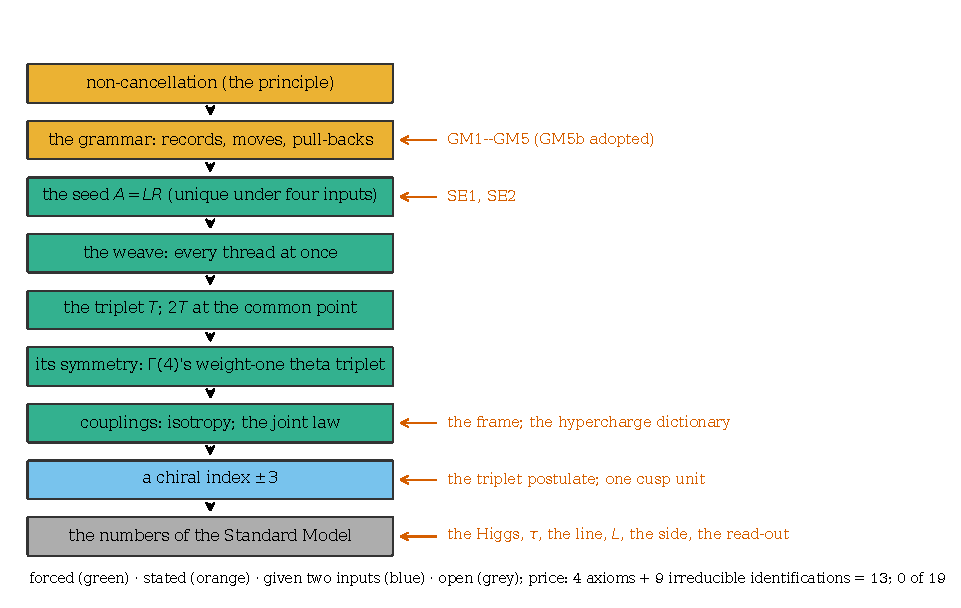
\includegraphics[width=0.92\linewidth]{figures/fig_chain}
\caption{The chain and its prices: what follows from the stated inputs of its section (green), what is stated (orange), what
also needs tagged postulates (blue), and what is open (grey). Inputs enter from the right. The seed is a side branch of
the grammar. A drawn schematic of Table~\ref{tab:inputs}.}\label{fig:chain}
\end{figure}

\paragraph{What is not.}
In the frames we studied, the same structure fixes none of the Standard Model's thirteen flavour numbers (\S\ref{sec:boundary}). The boundary
is as sharp as the forced half:
\begin{itemize}
\item in the frames where the inner automorphisms act, every residual subgroup of the weave's group either degenerates
  the masses or leaves them free, and none that reduces the count of mixing parameters is compatible with the CKM data
  at $3\sigma$;
\item no frame on record is shown to satisfy all of the principle's demands;
\item on the ruled branch the triplet's parameter-free coupling has $m_2/m_1\ge\tfrac12$ at every modulus
  (Corollary~\ref{cor:halffloor}), so it carries no hierarchy anywhere;
\item a sealed census finds that one Higgs at the symmetric point $\tau=\omega$ reproduces the five non-electron mass
  ratios on none of the admissible lines. The miss is the down--lepton ratio $(m_\mu/m_\tau)/(m_s/m_b)$, which the
  data put at $3.14$ (from $2.9$ to $3.4$ within the strange-quark mass's uncertainty alone);
\item whatever chooses the numbers is not given by the symmetry alone, although it acts at a symmetric point.
\end{itemize}

\paragraph{The motion.}
The grammar's states move. A random walk of steps and pull-backs escapes at a positive rate: for equal weights by the
theorems of Kesten and Furstenberg, and at the other weights by Furstenberg's theorem, since the support generates
$\SL(2,\Z)$; the values are measured. Two sealed arcs read that motion: B1663, and B1666, a scoreboard computed after
the gates of B1664 and B1665 had failed and their read-outs had been seen.
\begin{itemize}
\item The pull-back's strength sets the probability of the side the end lies on (from $1.000$ to $0.531$) and the speed, but not
  the defect it averages, to the test's resolution (B1663).
\item Averaged trace by trace, the threads approach the modular surface's constant mode ($0.3144$ at the largest
  traces against $0.31500491$, the gap shrinking as $t^{-0.51\pm0.05}$, a read-out): the weave side of the trace formula comes out where
  the wave side says, as equidistribution requires (a check of the instrument).
\item The amplitude built from the matter's defect returns after one period by the multiplier of $\eta^6$ (Theorem~\ref{thm:phase}). The normalised coherence of the cusp family $L^{4m+1}R$ climbs
  toward one, and the root $LR$ is not singled out (a read-out; the size of the coherent amplitude is not compared).
\end{itemize}
These are statements about the mathematics of the motion. We do not claim the motion is physical.

\paragraph{The record.}
The computations are archived in a public repository~\cite{OriginAxiomRepo}. A label such as B1659 names one
computation there (an \emph{arc}), with its preregistration, instrument, output and \emph{lock}, a test in the
repository's suite that fails if the result changes. A \emph{scoreboard} is a result computed on data that were already
seen, and is called so. A \emph{tagged} input is a working postulate whose results carry the word ``given''. The
program's work runs on several parallel lines on the same record; their cross-checks are internal to the program, not
external review.

\paragraph{The price.}
Every input is stated in Table~\ref{tab:inputs}, with what it buys and what would discharge it: the principle, the
grammar and the root's two conditions, one adopted reading, the choices (positivity, orientation, the boundary domain, the
frame, the modulus and the lines, the canonical horocycle, the hand and the $\eta$ twist, the Higgs's type and locus), the
tagged postulates, the readings (the weave's surface, the modular-flavour ansatz, the index formula), and the
identifications that turn structure into physics. No value of the Standard Model is derived:
none of its nineteen parameters. We built the computations as sealed tests: each preregistered,
run once per sealed version, and its output committed before it was read. The paper keeps its failures, including two failed gates of our own (\S\ref{sec:methods}).

\reading{The principle asks for something that cannot cancel. The grammar's answer is a motion: steps and their
pull-backs that never settle. The structure that motion carries holds on the stated inputs. What it leaves free is the choice of a
world.}

\section{The grammar and the seed}\label{sec:grammar}

\paragraph{The question.}
The principle says that existence is what remains when cancelling to nothing cannot complete. To ask what that forces,
the sentence has to be given a form in which something can be computed. This section gives it one: two records, two
moves and their pull-backs. It then asks the first question the form can answer, namely what the first description is
that mixes the two records and does not cancel. The answer is a theorem with four stated inputs, and the section
discloses how the answer was known before the inputs were written. All results of the program are cited by their
arcs in the repository~\cite{OriginAxiomRepo}.

\paragraph{The principle.}
We use the single wording of the record: existence is what remains when cancelling to nothing cannot complete (PF1);
that remainder is a description that cannot be exhausted (PF2); the program reads that description as mathematical
structure and asks what it forces (PF3). The three are postulated, as three faces of one commitment, and nothing in
the record derives one from another. The mathematical face of PF1 is a reading, not a derivation. For two letters $a,b$
of the once-punctured torus group it is the Fricke--Vogt invariant $\kappa=\tr[a,b]$, and cancelling to nothing
completes where $\kappa=2$. The wording is therefore that a description \emph{generically does not cancel}
($\kappa\neq 2$), never that it cannot.

\paragraph{The grammar.}
A \emph{description} is built from two integer records, $(a,b)\in\Z^2$. The grammar has five items.
\begin{itemize}
\item \emph{Records and moves} (GM1, GM2). An update acts on the pair of records. The elementary updates are the unit
  shears
  \[
    L=\begin{pmatrix}1&1\\0&1\end{pmatrix}:(a,b)\mapsto(a,a+b),\qquad
    R=\begin{pmatrix}1&0\\1&1\end{pmatrix}:(a,b)\mapsto(a+b,b),
  \]
  and a description is a word in them. Every hyperbolic class of $\SL(2,\Z)$ is, up to sign, a cyclic word in $L$ and $R$
  containing both letters (a classical fact~\cite{Series1985}; the paper's check \texttt{checks/positive\_words.py} confirms it for all $168$
  hyperbolic matrices with entries of absolute value at most $5$).
\item \emph{Aperiodicity} (GM3). The description does not repeat, so the monodromy is hyperbolic.
\item \emph{The carrier} (GM4). Words are realized as mapping classes of the once-punctured torus, whose first
  homology is $\Z^2$.
\item \emph{Reversible updates} (GM5a), with the unit shears of GM2.
\item \emph{The pull-back} (GM5b). The inverse moves $L^{-1}$ and $R^{-1}$ are legal updates.
\end{itemize}
GM5b is adopted as a reading of PF1's own cancelling, chosen on the mathematics (B1662); it is not a
derivation. In PF1's form $\kappa=\tr[a,b]$ the commutator is two letters followed by their two inverses. Among the
moves the same shape is the commutator of $LR$ and $RL$, which freely generate the commutator subgroup of $\SL(2,\Z)$,
the fundamental group of the modular once-punctured torus. This is classical; the paper's check script confirms it
(both words lie in the kernel of the abelianisation $\SL(2,\Z)\to\Z/12$, and a coset enumeration gives the subgroup they
generate index $12$).
Note that the commutator of the single letters is not of this kind: $\tr[L,R]=3$. The next two statements are the
facts the adoption rests on. Both are finite matrix computations.

\begin{proposition}[the failed cancellation and the sign]\label{prop:sign}
At the root the commutator of the two products $LR$ and $RL$ does not return to the identity. It equals $-U$ with $U$
unipotent, so its trace is $-2$: the cancellation lands on the cusp, with a sign. The sign itself is generated by the
moves and their pull-backs,
\[
  -I=(L\,R^{-1}L)^2=(L^{-1}R)^3 .
\]
\end{proposition}
\begin{proof}
Direct multiplication. $[LR,RL]=\begin{psmallmatrix}-7&6\\-6&5\end{psmallmatrix}=-U$ with $U=\begin{psmallmatrix}7&-6\\6&-5\end{psmallmatrix}$,
which has trace $2$ and is not the identity. Next, $L R^{-1}L=\begin{psmallmatrix}0&1\\-1&0\end{psmallmatrix}$ squares to $-I$, and
$L^{-1}R=\begin{psmallmatrix}0&-1\\1&1\end{psmallmatrix}$ has order six with cube $-I$. The square $(LR^{-1}L)^2=-I$ is unchanged when
$L$ and $R$ are replaced by their inverses (the mirror, B1662). The two elements fix the points $i$ and $\omega=e^{2\pi i/3}$ of the
upper half-plane, and no word in $L,R$ alone reaches them: a word in $L,R$ has non-negative entries, so $ad=1+bc\ge1$
forces $a,d\ge1$, and its trace is $2$ only when $a=d=1$, otherwise at least $3$; a finite order element has trace $0$ or
$\pm1$.
\end{proof}

The record reads the trace $-2$ through classical results and uses them only for what they say. On the character
variety of the once-punctured torus the trace of the commutator is $x^2+y^2+z^2-xyz-2$ in the traces
$(x,y,z)=(\tr a,\tr b,\tr ab)$ (Fricke's identity), and $-2$ is the value at which the commutator is parabolic: the
puncture. The modular group's action on these characters is studied in~\cite{Goldman2003}, and the classification of
the punctured-torus groups is in~\cite{Minsky1999}. We use the two references to name the setting and nothing more.

\paragraph{The direction of the moves.}
Three consequences of GM5b are readings, kept apart from the theorems.
\begin{itemize}
\item \emph{The sign is generated.} Proposition~\ref{prop:sign} shows that a full turn about a balance point negates
  both records. The place where a hand can be registered on a spin structure (B1479, B1481) is generated by the moves.
\item \emph{Positivity is the choice of side.} Step and pull-back are mirror images: conjugation by $\mathrm{diag}(1,-1)$
  sends $L$ to $L^{-1}$, $R$ to $R^{-1}$ and $\tau$ to $-\bar\tau$. The restriction to non-negative counts, which an
  earlier form of the grammar stated as a rule on states, is therefore a selection of one side of the mirror. It stays a
  chosen input. Under the pull-back the reachable updates are $\SL(2,\Z)$, and every hyperbolic class keeps a
  forward representative, so no statement about the threads changes.
\item \emph{The arrow is the escape.} A random walk with steps $L^{\pm1},R^{\pm1}$ at equal strength is transient on
  $\SL(2,\Z)$, since the group is non-amenable~\cite{Kesten1959}, and it escapes at a positive linear rate~\cite{Furstenberg1963,FurstenbergKesten1960}. These
  cover the symmetric walk; for the unequal weights of Section~\ref{sec:boundary} the rate is positive by Furstenberg's theorem, since the support
  generates $\SL(2,\Z)$, and its values are measured (B1663).
  The reading in which the pull-back only undoes the last step is recurrent at equal strength. So only the reading
  adopted here never settles at equal strength, and the arrow is the escape, a positive rate with no preferred side. We cite the two theorems and do not
  use the walk below until Section~\ref{sec:boundary}.
\end{itemize}

\paragraph{The seed.}
The first description that mixes the two records is a product of both unit moves. To see what the grammar selects, let
the increments of the shears vary: $L_a=\begin{psmallmatrix}1&a\\0&1\end{psmallmatrix}$, $R_b=\begin{psmallmatrix}1&0\\b&1\end{psmallmatrix}$ with
integers $a,b\ge1$, and set $B(a,b)=L_aR_b=\begin{psmallmatrix}1+ab&a\\b&1\end{psmallmatrix}$. The selection criterion SE1 asks that
the first homology of the mapping torus be torsion-free. Orientation (SE2) takes the orientable one of the two classes
that SE1 leaves.

\begin{theorem}[the seed, T1]\label{thm:seed}
Take GM3 (aperiodicity), GM4 (the once-punctured-torus carrier), SE1 (a torsion-free first homology) and SE2 (the
orientable choice). Then the root, the first mixed persistent sector, is the monodromy
\[
  A=LR=\begin{pmatrix}2&1\\1&1\end{pmatrix},\qquad \tr A=3,
\]
up to the order bit $LR$ against $RL$, and its mapping torus is the complement of the figure-eight knot. In
particular, on the positive grid $1\le a,b\le12$ all $144$ closures $B(a,b)$ are hyperbolic and exactly one is
torsion-free, $(a,b)=(1,1)$.
\end{theorem}
\begin{proof}[Proof (sketch; the record's uniqueness theorem, B1323, B1454)]
For $B\in\SL(2,\Z)$ one has $\det(B-I)=2-\tr B$, and the mapping torus has $H_1=\Z\oplus\mathrm{coker}(B-I)$. Hence for
$B(a,b)$: $\tr B=2+ab$, which exceeds $2$ for every $a,b\ge1$ (so all $144$ are hyperbolic), and the torsion of $H_1$
has order $ab$. It is trivial exactly when $ab=1$, that is $(a,b)=(1,1)$ and $B=LR$. On the full set of states, torsion
of order $|2-\tr|$ vanishes only for trace $3$ among the hyperbolic classes (GM3 excludes the elliptic trace $1$), and
the trace-$3$ class is that of $LR$ (the paper's check \texttt{checks/positive\_words.py} confirms it for every such matrix with entries up to $5$; the general
statement is the class-number-one fact for discriminant $5$~\cite{Buell1989}). When orientation-reversing monodromies are
admitted, the torsion has order $|\tr|$ and the torsion-free classes are those of $LR$ and of the golden matrix $LP$
(determinant $-1$, trace $\pm1$, with $(LP)^2=LR$), whose bundle is the Gieseking manifold $m000$. SE2 takes the
orientable one, $m004$, the orientation double cover of $m000$. The mapping torus of $LR$ is the figure-eight complement~\cite{Riley1975,Thurston1979}.
The words route (aperiodic $\Rightarrow$ Sturmian $\Rightarrow$ the golden matrix) and the records route are one
construction in two presentations (B1323; B1607 for the principle's tick).
\end{proof}

\noindent\emph{Scope.} The theorem is conditional on its four inputs, and each is needed: without GM3 the order-six
monodromy of trace $1$ (the trefoil complement) and the parabolic monodromies of trace $2$ also satisfy SE1; without GM4
the closed torus bundle of $LR$, which is torsion-free, remains; without SE1 every state remains; without SE2 the parent $m000$ remains. Positivity (the choice of the forward side), minimality of the trace, the unit-shear generation GM2 and
the order bit are not needed for the root. The root's uniqueness holds with and without positivity: without it the
torsion-free hyperbolic solutions are $(1,1)$ and $(-1,-1)$, in one class (B1454). The theorem selects one
\emph{thread} of the family that the grammar allows. It does not make that thread privileged, and no later result in
the paper uses it as a premise.

\begin{figure}[t]
\centering
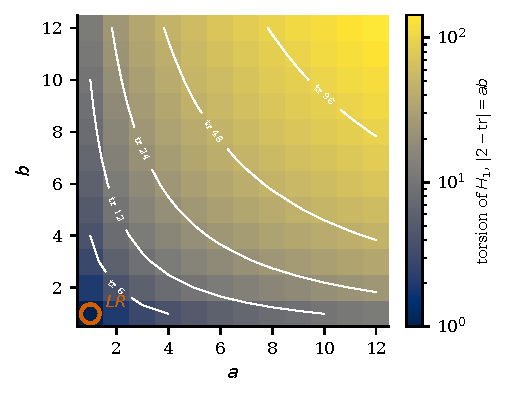
\includegraphics[width=0.62\linewidth]{figures/fig_seed}
\caption{An illustration of the identity $|H_1|=ab$, not a separate result. Torsion order $|2-\tr B(a,b)|=ab$ of $H_1$ over the $12\times12$ grid of
closures (colour, logarithmic), with contours of the trace $2+ab$. The root $LR$, $(a,b)=(1,1)$, is the only
torsion-free closure. This is an exact computation on the grid, conditional on the inputs of Theorem~\ref{thm:seed}.}
\label{fig:seed}
\end{figure}

\paragraph{Provenance.}
The root was known before the axioms were written: the figure-eight complement was named in a probe, and the grammar was
written afterwards. The genesis is therefore a conditional reconstruction of a chosen sector, not a derivation of the
figure-eight from nothing. We say so here because a reader will otherwise suspect it. No input of
Table~\ref{tab:inputs} is derived from a weaker one in the record, and none of the three further anchors proposed
within the program for the genesis is graded proved in the record (one is refuted, two are conditional).

\paragraph{The inputs.}
Table~\ref{tab:inputs} lists every input this paper uses, with its status, what it buys and what would discharge it. The
last lines of the table state the price as the record counts it.

{\footnotesize
\begin{longtable}{@{}p{3.2cm}p{2.4cm}p{3.6cm}p{6.0cm}@{}}
\caption{The inputs ledger. Status words follow the record: \emph{postulated}, \emph{chosen} (a selection),
\emph{adopted} (a ruling made on the mathematics), \emph{tagged} (a working postulate whose results carry ``given'').}\label{tab:inputs}\\
\toprule
input & status & what it buys & what would discharge it\\
\midrule
\endfirsthead
\toprule
input & status & what it buys & what would discharge it\\
\midrule
\endhead
\bottomrule
\endlastfoot
PF1--PF3, the principle & postulated & the question: what a non-cancelling description forces & none in the record\\
the grammar, GM1--GM5a & postulated (GM3 cheap; GM4's puncture conditional) & the moves, the threads, the carrier & none; GM1 is not independent of GM4\\
SE1, torsion-free first homology & postulated & the root among the states & alternatives are kept: minimal trace, minimal volume\\
SE2, orientation & chosen & the orientable root, and the sheet that carries the hand & a derived reason for orientability, or carrying both $m004$ and $m000$\\
GM5b, the pull-back acts & adopted, as a reading of PF1's cancelling & the sign $-I$ and a motion with no preferred side at equal strength; not needed for the root & not a derivation\\
positivity, as the side & chosen (a selection) & one side of the mirror: forward words & a reason for the side; what CP violation would read\\
the triplet postulate & tagged & left-handed matter in the triplet $T$; the mass tensor & a derivation of which fields carry $T$ (the dictionary), or an obstruction; an index for the count does not pay it\\
one cusp unit & tagged & the index $\pm3$ (Section~\ref{sec:three}) & an end mechanism at the cusp\\
the extreme boundary domain & chosen & $|\Lambda_+|\in\{0,6\}$, so $\pm3$ rather than $\pm1$ (Section~\ref{sec:three}) & a rule that selects the domain\\
$M_{1,2}$ as the weave's surface & a reading, verified in part & the setting of the index and of the zero modes & coherence of the lifts (a gate still open)\\
the vacuum-grading rule (demand D1, Section~\ref{sec:boundary}) & a ruling of the program & how a symmetry broken by a vacuum is graded & none\\
the end condition at the puncture (equal canonical amplitudes) and the choice of canonical horocycle & chosen (the horocycle a discrete choice; the radius of order one, Census law~\ref{cl:cusp}) & the norm of the boundary class, the lepton sector's null vector, the symmetric point's law, the census N5 and the first generation's lift (Sections~\ref{sec:couplings}, \ref{sec:three}) & an end mechanism at the puncture, or a reason for one horocycle\\
the modulus $\tau=\omega$ and the eighteen flat lines & chosen (a selection, Section~\ref{sec:selection}) & the lepton sector's null vector, the symmetric point and the one-Higgs census N5 (Sections~\ref{sec:couplings}, \ref{sec:boundary}) & a rule that selects the modulus and the lines\\
equal framed data & chosen & the twisted half bound & a reason that the sectors' framed data are equal\\
the index as the generation count & identification & reads the index $\pm3$ of Section~\ref{sec:three} as three generations & an index theorem on a physical spacetime\\
the read-out and the hypercharge dictionary & identifications & singular values as masses, flat-line twists as hypercharges and the Higgs line as the electroweak Higgs, with $6Y$ the minimal integral normalisation, itself a choice (Sections~\ref{sec:couplings}, \ref{sec:boundary}) & a derivation of the dictionary\\
the fibre frame (the Higgs a section on the fibre, at one $\tau$) & chosen (see Verdict~\ref{bd:tribunal}) & the couplings of Section~\ref{sec:couplings} & a frame shown to meet the demands\\
the Higgs's type and locus (a point or density Higgs, at the puncture) & stated & the covariance theorem and the rank of a point coupling (Section~\ref{sec:couplings}) & a Higgs of another type, or a derived locus\\
zero Wilson line on the fibre & stated (a restriction of the frame) & the isotropy theorem and its null vector (Section~\ref{sec:couplings}) & a derivation of the connection, or the theorem for a non-zero line\\
the hand and the $\eta$ twist & chosen conventions, not derived & $\rho$ as the theta multiplier (Section~\ref{sec:modular}) & a derived hand; a reason for the twist\\
the modular-flavour ansatz (holomorphic couplings, a minimal K\"ahler term, one copy of $T$ per field, one Higgs per sector) & stated where used, not adopted & the ruled-branch bound of Theorem~\ref{bd:reducesnone}; the half floor and the determinant laws of Section~\ref{sec:anomaly} (with real coefficients where the strong angle is read) & none\\
the moves as a symmetry of the fermions, with weights, and $\tau$ a field & stated where used & the anomaly of the moves and the strong angle's transformation (Section~\ref{sec:anomaly}) & a derivation that the moves act on the fermions as a symmetry\\
the Dedekind counterterm $\theta(\tau)=\theta_0+6K\arg\eta(\tau)$ & stated where used (an input with a field: $\mathrm{Re}\,\tau$ coupled to the gluons' $G\tilde G$) & a strong angle invariant under the moves (Proposition~\ref{prop:strong}) & a mechanism that supplies it, or weights with no anomaly\\
the index formula $\dim\Lambda_+-3$ & taken as stated (B1606) & the index of Section~\ref{sec:three} & an independent derivation\\
\midrule
\multicolumn{4}{@{}p{15.4cm}@{}}{\textbf{Price.} The rows above are this paper's inputs. For comparison, the
record's identification ledger, which prices the program's whole chain to the Standard Model including frames this paper
does not use, counts four axioms and nine irreducible identifications; this paper uses three of the nine (the triplet
postulate, the index as the generation count, and the read-out with its dictionary). The modulus $\tau$ and the
choice of canonical horocycle are not rows of that ledger. Against the Standard Model's nineteen values the paper derives
none.}\\
\end{longtable}}

\reading{The arena. SE1 has two solutions: trace $3$, the root, and trace $1$, the order-six move $L^{-1}R$ whose mapping
torus is the trefoil complement. Under the pull-back the second is reached by the moves (it fixes $\omega$), and GM3
keeps it from being a thread. We read the root as the motion and the trace-$1$ solution as the arena the motion
moves in: $\SL(2,\R)/\SL(2,\Z)$ is the complement of the trefoil~\cite{Milnor1971}, and the closed orbits of its
geodesic flow are the threads~\cite{Ghys2007}. The classical facts are cited, and nothing in the paper is derived from
this reading.}

\section{The weave}\label{sec:weave}

\paragraph{The question.}
The grammar allows many descriptions, not one. Section~\ref{sec:grammar} selected one of them as a root, under four
inputs. The honest form of the question ``what is forced'' is what holds for all the descriptions at once, with none
picked by hand. This section names the descriptions, names their joint action, and finds the first structure that the
joint action forces: the records' own parities, which move as three objects and which give a triplet. The program's
arcs are cited by number~\cite{OriginAxiomRepo}.

\paragraph{Threads.}
A \emph{thread} is a closed path of the moves through the shared records. Concretely it is a primitive hyperbolic
conjugacy class $\pm w$ in $\SL(2,\Z)$, where $w$ is a cyclic word in $L$ and $R$ containing both letters; such classes
exhaust the hyperbolic classes (Section~\ref{sec:grammar}). A thread is also a closed geodesic on the modular surface
$\Hb/\PSL(2,\Z)$, and the word is its cutting sequence~\cite{Series1985,Moeckel1982}. Its once-punctured-torus bundle is
a cusped hyperbolic $3$-manifold. The root $LR$ of Theorem~\ref{thm:seed} is one thread, of trace $3$.

\begin{definition}[the weave]\label{def:weave}
The \emph{weave} is the joint action of every allowed move on the records, together with everything that joint action
forces. A \emph{weave statement} takes every thread under a rule stated in advance, with none chosen, is defined by the
joint action, and is a claim about all threads at once. A \emph{thread statement} is anything read on one thread or on
its covers, and is labelled so.
\end{definition}

Every statement below is labelled in this way. Theorem~\ref{thm:seed} and the frames of the later sections are thread
statements. The next paragraphs are weave statements, and their ranges are stated: ``every thread'' always means every
thread in the stated range: every word where a proof is stated, and a stated bound on the word length where a census is.

\paragraph{Three, from parity.}
Reduce the records modulo $2$. The group $\SL(2,\mathbb{F}_2)$ acts on the three non-zero vectors of $\mathbb{F}_2^2$, the
three \emph{parities} $(1,0),(0,1),(1,1)$, as the symmetric group $S_3$. Nothing is put in to make three: $2^2-1=3$.

\begin{lemma}[the parity lemma]\label{lem:parity}
With the grammar's action $(a,b)\mapsto(a,a+b)$, $L$ fixes the parity $(0,1)$ and exchanges the other two; $R$
fixes $(1,0)$; the swap $P:(a,b)\mapsto(b,a)$ of the two records (not a move of
the ruled grammar; see below) fixes $(1,1)$; the sign $-I$ fixes all three. Any two of $L$, $R$ and the swap generate $S_3$ on the three
parities. For $\phi\in\SL(2,\Z)$, $\tr\phi$ is odd if and only if $\phi$ acts on the parities as a $3$-cycle.
\end{lemma}
\begin{proof}
Modulo $2$, $L$ and $R$ are the transvections $\begin{psmallmatrix}1&1\\0&1\end{psmallmatrix}$ and $\begin{psmallmatrix}1&0\\1&1\end{psmallmatrix}$, which are transpositions of the three
non-zero vectors; two distinct transpositions generate $S_3$. An element of $\SL(2,\mathbb{F}_2)$ of order three has
characteristic polynomial $x^2+x+1$, hence trace $1$; the identity and the transpositions have trace $0$.
\end{proof}

The lemma is exact for every word. The record also checked it on all $988$ signed words to length eight ($448$ of odd
trace; B1600). Thus the three parities are cycled by every thread of odd trace, with no thread chosen, and a thread of
even trace fixes at least one of them.

\paragraph{The common point.}
For a thread, take the traces $(x,y,z)=(\tr a,\tr b,\tr ab)$ of the fibre's holonomy at the geometric point. The
Fricke maps of $L$ and $R$ act on the parabolic surface $x^2+y^2+z^2=xyz$ (commutator trace $-2$, the puncture), and on this
surface their only common fixed point is the origin $(0,0,0)$, the \emph{quaternion point}: there the holonomy sends
$a\mapsto i$ and $b\mapsto j$ in the quaternion group $Q_8\subset\mathrm{SU}(2)$ (B1600, W2). We call it the
\emph{common point}. It is the point at which every odd-trace thread meets the same finite picture.

The common point is also the geometry modulo three. For a thread with odd trace the ideal generated by $(x,y,z)$ in the
ring of integers of $\mathbb{Q}(x,y,z)$ is, on every thread to word length eight, one prime of residue degree one above
$3$, of norm $3$ and multiplicity one. The holonomy reduces modulo that prime to the quaternion point, and the cover
that forces the binary tetrahedral group $2T=\SL(2,\mathbb{F}_3)$ is the thread's principal congruence cover at it. For
even trace the ideal is a power of a prime above $2$, and the common point is the trivial representation (B1601).

\begin{censuslaw}[the geometry modulo three, B1601]\label{law:modthree}
Call a \emph{geometry} the bundle of a thread up to the symmetries that preserve it (cyclic rotation and the exchange of $L$
and $R$), so that each is computed once. On all $37$ geometries of word length at most eight ($16$ of odd trace, $21$ of even trace), an odd-trace thread has the
prime above $3$ described above, and an even-trace thread has no prime above $3$. The linearized lemma behind it is
proved: the Fricke maps' linear parts at the common point are quarter turns about the $x$- and $y$-axes of the three
parity lines, generating the rotations of the cube, and a word has odd trace if and only if its linear part is a
third turn about a body diagonal, an axis isotropic for $x^2+y^2+z^2$ exactly in characteristic three. That odd trace
\emph{always} gives this prime, and even trace never, is not proved for all words.
\end{censuslaw}

\paragraph{The parity triplet.}
The moves act on the three parities, and the common point carries $2T$. Together they give a triplet.

\begin{theorem}[the parity triplet, T2]\label{thm:triplet}
\begin{enumerate}
\item \textbf{(Parity.)} The moves act on the three non-zero parities of the two records as $S_3$, and a thread has odd
  trace if and only if it acts as a $3$-cycle (Lemma~\ref{lem:parity}; every word).
\item \textbf{(The common point.)} For every odd-trace word, there is an element $\tau\in2T\setminus Q_8$ conjugating
  $(i,j)$ to the images of the thread's generators, and the group generated by $i,j,\tau$ is $2T$, of order $24$. The group
  acts on the three parity lines as the standard three-dimensional irreducible representation of $A_4=2T/\{\pm1\}$
  (character $(3,-1,0,0)$, norm one). For an even-trace word the conjugator lies in $Q_8$ if the word acts trivially on the
  parities, and in the binary octahedral group $2O$ outside $2T$ if it acts as a transposition; the parity lines split.
  The arithmetic of the common point, a prime above $3$, is Census law~\ref{law:modthree}.
\item \textbf{(The zero modes.)} On the weave's surface $M_{1,2}$ (taken as a reading, Table~\ref{tab:inputs}), let $V$ be
  the parity-twisted spin space. The group generated by the lifts of $L$ and $R$ on $V=T\oplus\bar T$ has order $96$. The
  Hodge--Riemann form on $V$ is invariant under $L$, $R$ and the sign, has signature $(3,3)$ and is positive definite on
  $T$. The punctured fibre with this local system has three holomorphic zero modes, one per parity, and they span $T$.
\end{enumerate}
\end{theorem}
\begin{proof}[Proof (records B1600, B1606, B1624)]
(1) is Lemma~\ref{lem:parity}. (2) The Fricke maps fix the common point, so for a word $\varphi$ the representation $\rho\circ\varphi$ of the free
group, with $\rho(a)=i$ and $\rho(b)=j$, has the character of $\rho$. It is irreducible, so $\rho\circ\varphi=g\rho g^{-1}$
for some $g\in\mathrm{SU}(2)$, determined up to sign. Then $g$ normalises $Q_8$, so $g$ lies in $2O$, the normaliser of
$Q_8$ in $\mathrm{SU}(2)$. The class of $g$ in $2O/Q_8\cong S_3\cong\mathrm{Out}(Q_8)$ is the action of $\varphi$ on the parities.
So $g\in2T\setminus Q_8$ exactly when the trace is odd (Lemma~\ref{lem:parity}), $g\in Q_8$ when $\varphi$ is trivial
modulo $2$, and $g\in2O\setminus2T$ for a transposition; for odd trace $\langle i,j,g\rangle=2T$. The record checks this with
exact rational quaternion matrices for every word of length at most six (B1600); the first attempt with irrational entries
failed an equality test because of an error in the instrument, caught by an impossible group order and corrected before
anything was read off. The triplet is then a statement of representation theory:
$h^1(F;\chi_\varepsilon)=1$ for each non-zero parity $\varepsilon$ (the twisted cohomology of the punctured torus), and
$A_4=(\mathbb{Z}/2)^2\rtimes\mathbb{Z}/3$ permutes the three non-trivial characters of $(\mathbb{Z}/2)^2$ cyclically,
which is the standard irreducible three. For an involution the representation splits. (3) Here $V=\bigoplus_p H^1(F;\chi_p\otimes\rho_Q)$, with $\rho_Q(a)=i$, $\rho_Q(b)=j$ the
common point's quaternion representation and $\chi_p$ the parity character. A move $m$ lifts through the element $g$ of
$2O$ with $\rho_Q\circ m=g\rho_Q g^{-1}$: $g_L=(1+i)/\sqrt2$ for $L\colon a\mapsto a,\ b\mapsto ab$, and
$g_R=(1-j)/\sqrt2$ for $R\colon a\mapsto ab,\ b\mapsto b$. The cup product on the
$\mathbb{Z}/2$-orbifold presentation of the fibre group, by an independent implementation, gives the form and its
signature; the zero modes are $F=(f(z),f(z+\tau))\,dz$ with $f=\theta_3(z;2\tau)/\sqrt{\theta_1(z;\tau)}$ and the three
parity twists $F_p=C_pF$, with $C_p$ the unit of $Q_8$ attached to the parity $p$ and the square root continued along
the segments that represent $a$ and $b$, so that $F$ has the monodromy of $\rho_Q$ (W21).
\end{proof}

\noindent\emph{Scope.} Parts (1) and (2) are theorems: weave statements for every word, with no bound on the length. The
prime above $3$ of Census law~\ref{law:modthree} is a census. Part (3) holds on the
surface $M_{1,2}$, whose identification with the weave's object is a reading made within the program, of which only the
Euler characteristic is verified ($\chi=1/12$ by two routes; B1624). The identification of the zero modes with
left-handed matter is a further reading and is not used here. The index of the puncture (odd, never zero, and $\pm3$
once the parity grading is kept, B1606) belongs to Section~\ref{sec:three}. The triplet is a flavour structure: the
record grades the flavour three as derived on the weave and the gauge three as a selection, and the paper claims the first
only. The verification of (1)--(3) in the record is B1600 and B1606.

\paragraph{What is classical.}
A triplet of $A_4$ on three lines permuted by an order-three element is the standard flavour triplet of discrete flavour
models; we cite the use and not the construction~\cite{MaRajasekaran2001,AltarelliFeruglio2005}. What the weave adds is that the three lines, the group and the
irreducibility come from the records' parities and the common point, with no choice of group: proved for every odd-trace
word.

\begin{remark}[the moves that are not there]
The swap of the two records and the inner automorphisms of the free group by $a$ and $b$ are not moves of the
grammar adopted here. This matters in Section~\ref{sec:modular}: the group $\langle L,R\rangle\cong B_3$ meets
$\mathrm{Inn}(F_2)$ only in $\langle\Delta^4\rangle$, so the weave's group is the braid group, not its extension by the
point-pushes. Results of the program that take the inner automorphisms as symmetries hold on branches that add them, and
say so (B1634, B1640).
\end{remark}

\paragraph{One example.}
The root's own triplet is the running example of the paper. Its trace $3$ is odd, so $LR$ cycles the three parities, its
common point is the quaternion point, and its three parity lines form the standard triplet of $A_4$. It is one of the
odd-trace threads of Theorem~\ref{thm:triplet}, with no property, for the triplet, that the others lack.

\section{The triplet is modular}\label{sec:modular}

\paragraph{The question.}
The triplet of Section~\ref{sec:weave} is acted on by the moves. The next question is what that action is. If it were
an arbitrary finite group, the triplet would carry no further structure. We find instead that the action is the
multiplier of a classical family of theta functions: the grammar's moves, with no modular input, reproduce the level-four
theta multiplier that modular flavour models use, up to a twist by a power of the eta character. The twist doubles the
image from order $48$ to order $96$ and moves the allowed weights to $3/2$ modulo $2$ (Theorem~\ref{thm:theta}). The record is cited by arc~\cite{OriginAxiomRepo}, and what is known is
cited where it is used.

\paragraph{The setting.}
Take the moves on the ruled branch, that is $\langle L,R\rangle$ with no swap and no sign move beyond those generated
(Section~\ref{sec:grammar}). This group is the braid group $B_3$, acting on the once-punctured torus group $F_2=\langle
a,b\rangle$, and it maps onto $\SL(2,\Z)$ with kernel $\langle\Delta^4\rangle$, where $\Delta^{-1}=RL^{-1}R$ and
$\Delta^2\mapsto-I$ on homology. The metaplectic group is $\mathrm{Mp}_2(\Z)=\langle s,t\mid s^2=(st)^3,\ s^8=1\rangle=B_3/\langle\Delta^8\rangle$.
Write $s$ and $t$ for the images of $RL^{-1}R$ and $L$ in $B_3/\langle\Delta^8\rangle=\mathrm{Mp}_2(\Z)$.

\begin{proposition}[the inner automorphisms are not moves, B1634]\label{prop:inner}
The group $\langle L,R\rangle\cong B_3$ meets $\mathrm{Inn}(F_2)$ exactly in $\langle\Delta^4\rangle=\langle\mathrm{conj}(c)\rangle$, $c=a\,b^{-1}a^{-1}b$.
To word length $12$ the words acting on $F_2$ as inner automorphisms are $1{,}944$ relators (the identity), $196$ words for
$\mathrm{conj}(c)$ and $196$ for its inverse, and none for $\mathrm{conj}(a^{\pm1})$ or
$\mathrm{conj}(b^{\pm1})$. Every word acting on $F_2$ as an inner automorphism lifts to a scalar on the triplet.
\end{proposition}
\noindent\emph{Proof and scope.} The intersection is the classical kernel of $B_3\to\SL(2,\Z)$ acting on $\pi_1$ of the
punctured torus, and the census to length $12$ is exact (B1634, a verification of a claim made within the program). The
statement is about the ruled branch only. On branches that add the sign move or the swap, or give the records' base
point moves of its own, the inner automorphisms act, and results that use them are stated there.

\paragraph{The multiplier.}
Let $T$ be the triplet of Theorem~\ref{thm:triplet}, with the lifts of the moves defined on $V=T\oplus\bar T$ by the
parity-twisted action of Section~\ref{sec:weave}. We write $\rho$ for the representation of the moves on $T$,
$\rho(\gamma)=\mathrm{lift}(\gamma)^{-1}$; this is the convention in which $T$ is cohomology, so its monodromy is
the pull-back's inverse. The theta constants are $\theta_2,\theta_3,\theta_4$ in the nome $q=e^{i\pi\tau}$, and
$u=(\theta_2^2,\theta_3^2,\theta_4^2)$ satisfies Jacobi's identity $\theta_3^4=\theta_2^4+\theta_4^4$. Its components are
modular forms of weight one on $\Gamma(4)$, and the graded ring of the modular forms of $\Gamma(4)$ is generated by them
modulo that one relation. Both sides have dimension $2d+1$ in weight $d$: $\Gamma(4)$ has genus zero and six regular
cusps~\cite[ch.~3]{DiamondShurman2005}, and the quotient of the polynomial ring by the irreducible quadric injects
because the image has Krull dimension two. Modular flavour models use this ring as their
input~\cite{NovichkovPenedoPetcov2021,LiuYaoDing2020}. The transformation laws of the theta constants,
the theta functions with characteristics on the torus, are classical~\cite{WhittakerWatson1927,AlvarezGaumeMooreVafa1986}.
We write $\rho_u$ for the multiplier of the vector $u$ under $\mathrm{Mp}_2(\Z)$; it is trivial on $\Gamma(4)$, and
$\chi_\eta$ for the multiplier character of the Dedekind eta function.

\begin{theorem}[the theta multiplier, T3]\label{thm:theta}
Take the ruled weave on the triplet $T$ in the convention above.
\begin{enumerate}
\item The lifts of the moves satisfy the braid relation and send $\Delta^4$ to $-I$. They are therefore a genuine
  (not projective) representation $\rho$ of $B_3/\langle\Delta^8\rangle=\mathrm{Mp}_2(\Z)$.
\item $\rho$ equals, with no rescaling, the multiplier of the vector $\eta^{21}\cdot(\theta_2^2,\theta_3^2,\theta_4^2)$:
  \[
    \rho=\chi_\eta^{21}\otimes\rho_u ,
  \]
  the weight-one multiplier $\rho_u$ of the $\Gamma(4)$ triplet twisted by a power of the eta character. The intertwiner
  from the parity lines to the theta constants is monomial: $\theta_3^2$ lies on the clock's line (the parity
  character $(-,-)$), $\theta_2^2$ on the line $(+,-)$, and $\theta_4^2$ on the line $(-,+)$. (A line is labelled by the
  signs of its character on $a$ and $b$. Lemma~\ref{lem:parity}, Appendix~\ref{app:hand}'s row-vector right action and
  the record's pull-back of characters share these labels: $L$ fixes the parity $(0,1)$, the line $(+,-)$, and $R$ fixes
  $(1,0)$, the line $(-,+)$. The labels $(+,-)$ and $(-,+)$ exchange only under left multiplication of column vectors.)
  The exponents of $t$ on $T$ are
  $(\tfrac18,\tfrac38,\tfrac78)$ turns.
\item The dimension of the space $M_k(\rho)$ of vector-valued forms of weight $k$ for $\rho$ is
  $0,0,1,1,2,2,3,3$ at the allowed weights $k=-\tfrac12,\tfrac32,\tfrac72,\dots,\tfrac{27}{2}$ (step $2$; a weight is
  \emph{allowed} when the central element acts consistently with it, a necessary condition, not the existence of a
  form). In particular $\dim M_{3/2}(\rho)=0$: weight $\tfrac32$ is allowed and carries no form. The dual
  representation is not allowed at weight $\tfrac32$.
\end{enumerate}
\end{theorem}
\begin{proof}[Proof sketch (record B1634, with B1640's convention scoping)]
(1) The spin lifts of the moves are elements of the binary octahedral group $2O\subset\mathrm{SU}(2)$ (B1634). Acting on
$V=T\oplus\bar T$ through the parity twist they generate a finite group of order $96$, which acts faithfully on $T$
because $T$ and $\bar T$ have the same kernel (B1600). The braid relation holds exactly: $g_Lg_R^{-1}g_L=g_R^{-1}g_Lg_R^{-1}=(i+j)/\sqrt2$ in $2O$ for the spin lifts
$g_L=(1+i)/\sqrt2$ and $g_R=(1-j)/\sqrt2$, and $LR^{-1}L=R^{-1}LR^{-1}$ in $\mathrm{Aut}(F_2)$ (the record also checks it
numerically, to $3\cdot10^{-16}$); and $\Delta^4$, the generator of the kernel, acts as $-1$ (turns $\tfrac18,\tfrac18,\tfrac58$ for the
lift of $\Delta$). The lifts compose in reverse, so $\rho=\mathrm{lift}^{-1}$ is a homomorphism. (2) With $s,t$ as above,
$\rho(s)$ and $\rho(t)$ satisfy $s^2=(st)^3$ and $s^8=1$ exactly, so $\rho$ is a representation of $\mathrm{Mp}_2(\Z)$. The
theta transformation laws, evaluated from the series in $\tau$ at several points, fix $\rho_u$, and a linear solve for an
intertwiner with $\rho$ returns an intertwiner with no rescaling (both scale factors equal to $1$) and smallest singular value $1.5\cdot10^{-15}$; its monomial shape is
exact. Four of the eight identifications of $(s,t)$ with the generators and their inverses need no rescaling, and two of
them are allowed at weight $3/2$. The record's sealed check of the classical laws failed at one of its two points (the
$T$ law off by a relative $1.10$ at $\tau=0.13+1.21i$); it was traced to the instrument's principal branch of $q^{1/4}$,
and at the other point both laws hold to $2\cdot10^{-15}$ (B1634, disclosed there). (3) If $f\in M_k(\rho)$ then $\eta^3f$ is a form of weight $k+\tfrac32$ for the
multiplier of $u$ vanishing at the cusp, and the converse holds; the forms of $\Gamma(4)$ are the polynomials in $u$
modulo the one relation ($2d+1$ of them in degree $d$), and the count is exact linear algebra. At $k=\tfrac32$ the only
candidate is the Serre derivative of $u$, whose constant term $-\tfrac1{12}(0,1,1)$ does not vanish, so it gives no form
and $\dim M_{3/2}(\rho)=0$. As a cross-check, the counts above weight $2$ agree with the dimension given by the
Selberg trace formula~\cite[\S7]{Borcherds2000}. Below weight $2$ the same expression is only an Euler characteristic,
$\dim M_k(\rho)-\dim S_{2-k}(\rho^\vee)$; at $k=\tfrac32$ it is $0$, and both terms vanish.
\end{proof}

\noindent\emph{Scope.} Four limitations are part of the statement.
\begin{itemize}
\item \emph{What is classical, what is automatic and what is computed.} The modular group permutes the three even theta
  characteristics of the torus through $\SL(2,\mathbb F_2)\cong S_3$, and the theta multiplier of Section~\ref{sec:modular}'s
  setting is classical. Two genuine representations of $\mathrm{Mp}_2(\Z)$ that agree projectively differ by a character,
  and the characters of $\mathrm{Mp}_2(\Z)$ are the powers of $\chi_\eta$ (its abelianisation is $\Z/24$). So once the
  parity lines are identified with the even characteristics, a power of $\chi_\eta$ is automatic. What the theorem
  computes is the projective agreement (the relative phases of the monomial matrices), the exponent $21$, and with it the
  central character that allows weight $\tfrac32$; it computes a stated lift, not a derived flavour symmetry.
\item \emph{The hand is a convention.} Writing $\rho=\mathrm{lift}^{-1}$ is one of two homomorphisms; the other is the
  complex conjugate, and the choice of which piece of $V$ is called $T$ is a second binary choice. The two together
  select $\rho$ or $\bar\rho$. The representation is irreducible and not equivalent to its conjugate (an independent exact
  audit, B1640). The record's choice has weight $3/2$ allowed (in the sense above; no form exists there) and admits the lowest
  symmetric weight-one coupling (B1640); the conjugate has neither. So the index and that coupling come with the same hand,
  and which hand the matter carries is not derived here. The hand's functorial reason (cohomology pulls back) is a
  reading of the record, not a theorem of this section.
\item \emph{The eta twist.} The theorem identifies $\rho$ with the theta multiplier up to the one-dimensional character
  $\chi_\eta^{21}$; it is not the bare weight-one multiplier of $\Gamma(4)$'s triplet. The restriction of $\rho$ to $\Gamma(4)$ is that
  character. We do not claim that the twist is forced rather than a convention of the homology generators.
\item \emph{The dimension formula.} The identification of the forms of $\Gamma(4)$ with the polynomials in $u$ modulo
  Jacobi's identity holds in every degree $d$ by the argument in the setting above (injectivity, and dimension $2d+1$ on both
  sides). It rests on the standard dimension formula $2d+1$ for the genus-zero curve with six regular cusps; it was also
  certified numerically for $d\le5$.
\end{itemize}

\begin{remark}[the modulus breaks the weave's group]\label{rem:modulus}
On the ruled branch the weave forces no point of the upper half-plane. At a generic $\tau$ the stabilizer of $\tau$ in
$\langle L,R\rangle$ is the centre, so the residual symmetry on $T$ is four scalars. At $\tau=i$ it is cyclic of order $8$,
a plane containing the clock's line and a line in the span of the letters' two lines; at $\tau=\omega=e^{2\pi i/3}$ it is cyclic of order $12$, with
three eigenlines, each with squared overlap $\tfrac13$ with every parity line (B1634). Consequently the modulus $\tau$ is the state that
breaks the weave's group. On the modular-flavour ansatz (holomorphic couplings, a minimal K\"ahler term, one copy of $T$
per field, one Higgs per sector), which this paper uses only for the ruled-branch bound of Theorem~\ref{bd:reducesnone},
the flavour numbers would be the values of vector-valued modular forms for $\rho$ at $\tau$. The couplings of
Section~\ref{sec:couplings} are built from such forms together with norms that are not holomorphic, so they are not of that
kind. The
statements of the earlier record that used the inner automorphisms as symmetries (an order-48 residual at $\omega$, a
permutation mixing for every $\tau$) hold on the branches where those act and not on the ruled branch.
\end{remark}

\subsection{The lowest couplings, the determinant character and the strong angle}\label{sec:anomaly}

This subsection works on the ruled branch with the modular-flavour ansatz of Remark~\ref{rem:modulus}, with one singlet
Higgs of weight zero, so that a sector's coupling between fields carried by $\rho_L$ and $\rho_R$ is a form in
$M_k(\rho_L^\vee\otimes\rho_R^\vee)$: odd $k$ when both fields carry $T$, even $k$ when one carries $\bar T$. The
statements about the strong angle add one input, the moves as a symmetry of the fermions (Table~\ref{tab:inputs}).

\begin{corollary}[the half floor at weight one, B1635, B1636]\label{cor:halffloor}
With every field in $T$, the coupling of weight one is unique up to a constant (B1635) and is the theta constants placed
off the diagonal,
\[
  Y_1\propto\begin{pmatrix}0&\theta_4^2&\theta_3^2\\ \theta_4^2&0&\theta_2^2\\ \theta_3^2&\theta_2^2&0\end{pmatrix}.
\]
Its singular values $s_1\ge s_2\ge s_3$ satisfy $s_1=s_2+s_3$ at every $\tau$, so $s_2/s_1\ge\tfrac12$ at every
$\tau$. The spectrum is $(1,\tfrac12,\tfrac12)$ at $\omega$ and $(1,\varphi^{-1},\varphi^{-2})$ at $i$. With one form per
sector, $M_u\propto M_d$ and the mixing matrix is the identity.
\end{corollary}
\begin{proof}
For a complex symmetric matrix with zero diagonal, the elementary symmetric functions of the eigenvalues of $YY^\dagger$
satisfy $e_1^2=4e_2$, a polynomial identity in the three entries (checked symbolically). In terms of the singular values
this is $(s_1+s_2+s_3)(-s_1+s_2+s_3)(s_1-s_2+s_3)(s_1+s_2-s_3)=0$, so the largest is the sum of the other two, and
$s_2\ge s_3$ gives $s_2\ge s_1/2$. The coupling's form and the spectrum at $i$ and on the tick's geodesic are B1636's,
and the sum rule for every coupling of that piece is its census G2. At $\omega$ the three theta constants have equal
moduli, since $\lambda(\omega)=e^{i\pi/3}$ gives $|\theta_2^4|=|\theta_4^4|=|\theta_3^4|$; the spectrum computed there
is $(1,\tfrac12,\tfrac12)$.
\end{proof}
\noindent\emph{Scope.} The floor is a statement about the ruled branch's parameter-free coupling under the ansatz; the
data need $m_2/m_1$ below $0.06$ in every charged sector. With $R$ in $\bar T$ the coupling of weight zero is the
identity, three degenerate masses (B1635). In the fibre frame the floor $\tfrac12$ of Theorem~\ref{thm:isotropy}(2)
holds for real Higgs directions only; complex directions reach any ratio near the isotropic cone. So the floor is not a
property of every frame.

\paragraph{The determinant character.}
\begin{proposition}[the determinant character, B1674]\label{prop:detchar}
$\det\rho=\chi_\eta^{9}$.
\end{proposition}
\begin{proof}
A character of $\mathrm{Mp}_2(\Z)$ is fixed by its value on $t$, whose image generates the abelianisation $\Z/24$, and
$\chi_\eta(t)=e^{2\pi i/24}$. By Theorem~\ref{thm:theta}(2) the exponents of $t$ on $T$ sum to $\tfrac18+\tfrac38+\tfrac78
=\tfrac{11}8\equiv\tfrac{9}{24}$ turns. The value on $s$ agrees (B1674).
\end{proof}

\paragraph{The moves' anomaly.}
Suppose the moves act on the Standard Model's fermions as a symmetry. Each multiplet $f\in\{Q,u^c,d^c,L,e^c\}$, and
$\nu^c$ where it is named, carries its three generations in $T$ ($s_f=+1$) or in $\bar T$ ($s_f=-1$). A modular
transformation then rotates the left-handed fermions, and the rotation shifts the angle of each gauge factor $G$ by its
anomaly. At the level of the character the shift is the character $\chi_\eta^{n_G}$, with
\[
  n_G(s)=9\sum_f w_G(f)\,s_f\pmod{24},
\]
where $w_G(f)$ is twice the Dynkin index of $f$'s representation of $G$ times its multiplicity under the other factors:
$(w_Q,w_{u},w_{d})=(2,1,1)$ for $\mathrm{SU}(3)^2$, $(w_Q,w_L)=(3,1)$ for $\mathrm{SU}(2)^2$, and the dimensions
$(6,3,3,2,1,1)$ for gravity.

\begin{proposition}[the anomaly of the moves, B1674]\label{prop:anomaly}
Given the triplet postulate and the moves as a symmetry of the fermions, at the level of the character:
\begin{enumerate}
\item the mixed anomaly with $\mathrm{SU}(3)$ vanishes exactly when $s_u=s_d=-s_Q$, that is, when the moves act on the
  left-handed and the right-handed quarks by the same representation (16 of the 64 assignments);
\item the mixed anomaly with $\mathrm{SU}(2)$ never vanishes: $n_{\mathrm{SU}(2)}\in\{6,12,18\}$;
\item among the assignments of (1), the gravitational anomaly vanishes exactly when $s_e=s_\nu=-s_L$, and without
  $\nu^c$ it never vanishes.
\end{enumerate}
\end{proposition}
\begin{proof}
Since $3$ is invertible modulo $8$, $n_G\equiv0\pmod{24}$ exactly when $\sum_f w_G(f)s_f\equiv0\pmod 8$. In (1) the sum
$2s_Q+s_u+s_d$ lies in $\{0,\pm2,\pm4\}$ and vanishes exactly as stated. In (2) the sum $3s_Q+s_L$ lies in
$\{\pm2,\pm4\}$. In (3), given (1), the sum is $2s_L+s_e+s_\nu$, which vanishes exactly when $s_e=s_\nu=-s_L$; without
$\nu^c$ it is odd. B1674 enumerates the 64 assignments exactly.
\end{proof}

\paragraph{The couplings' determinants and the strong angle.}
The strong angle is $\bar\theta=\theta-\arg\det(M_uM_d)$, with $M=Yv$. With one singlet Higgs its phase cancels from
$\bar\theta$, and a move shifts $\bar\theta$ by the phase of the multiplier of $\det(Y_uY_d)$. That is the anomaly of
Proposition~\ref{prop:anomaly} together with the cocycle of the weights.

\begin{proposition}[the determinants and the strong angle, B1674]\label{prop:strong}
Let the up and down couplings have weights $k_u,k_d$, and put $K=k_u+k_d$.
\begin{enumerate}
\item $\det(Y_uY_d)$ is a form of weight $3K$ with character $\chi_\eta^{m}$, $m=-9(2s_Q+s_u+s_d)$. It is $\eta^{6K}$ times
  a modular function exactly when $6K\equiv m\pmod{24}$:
  \begin{itemize}
  \item for every quark in $T$, exactly when $K\equiv2\pmod 4$;
  \item for $s_u=s_d=-s_Q$, exactly when $K\equiv0\pmod 4$;
  \item for the mixed assignments, when $K\equiv1$ or $3\pmod4$, by the hand.
  \end{itemize}
  When it holds, a counterterm $\theta(\tau)=\theta_0+6K\arg\eta(\tau)$, which we call the Dedekind counterterm, makes
  $\bar\theta$ invariant under the moves, and $\bar\theta-\theta_0=-\arg g$ with $g=\det(Y_uY_d)/\eta^{6K}$.
\item At weight one with every quark in $T$, $\det Y_1=2\theta_2^2\theta_3^2\theta_4^2=8\eta^6$. With real coefficients
  and no counterterm, $\bar\theta-\theta\equiv-12\arg\eta(\tau)\pmod\pi$. This is $-\pi\,\mathrm{Re}\,\tau$ up to terms
  of order $e^{-2\pi\,\mathrm{Im}\,\tau}$, and it is $\pi/2$ exactly on $\mathrm{Re}\,\tau=\tfrac12$. With the counterterm,
  $g$ is constant, so $\bar\theta$ takes one value at every $\tau$.
\item At weight three with every quark in $T$, and at weight two with $s_u=s_d=-s_Q$, each sector's determinant is a
  constant times $\eta^6E_6$, and a constant times $E_6$, respectively.
  \begin{itemize}
  \item With the counterterm, $g$ is a constant times $E_6^2/\Delta=j-1728$. With real coefficients, $\bar\theta-\theta_0$
    is a multiple of $\pi$ exactly on the imaginary axis and on the boundary of the fundamental domain. These are the
    loci where generalised CP is conserved in modular models~\cite{NovichkovPenedoPetcovTitov2019}, and there the mixing
    phase vanishes.
  \item Without the counterterm, at weight three, $\bar\theta-\theta\equiv-(12\arg\eta+2\arg E_6)\pmod\pi$. This vanishes
    on the imaginary axis and also on a curve inside the fundamental domain: from $\mathrm{Re}\,\tau\approx0.324$ at
    $\mathrm{Im}\,\tau=1$ to $\mathrm{Re}\,\tau\approx0.172$ at $\mathrm{Im}\,\tau=1.2$.
  \end{itemize}
\end{enumerate}
\end{proposition}
\begin{proof}[Proof sketch]
(1) The coupling transforms as $Y(\gamma\tau)=(c\tau+d)^k\rho_L^\vee(\gamma)Y(\tau)\rho_R^\vee(\gamma)^{T}$, so its
determinant carries $(c\tau+d)^{3k}(\det\rho_L\det\rho_R)^{-1}$, and Proposition~\ref{prop:detchar} gives $m$. The power
$\eta^{6K}$ carries $\chi_\eta^{6K}(c\tau+d)^{3K}$, so the quotient has weight zero and trivial character exactly when
$6K\equiv m$.

(2) The determinant of a zero-diagonal symmetric matrix is twice the product of its entries, and
$\theta_2\theta_3\theta_4=2\eta^3$~\cite{WhittakerWatson1927}; the identity and the phase law are also checked
independently in B1671. On $\mathrm{Re}\,\tau=\tfrac12$ the nome
$e^{2\pi i\tau}$ is negative, so $\eta^{12}$ is $i$ times a positive number.

(3) The quotient of the determinant by $\eta^6$, or the determinant itself, is a form of weight six for $\SL(2,\Z)$:
its exponents at the cusp are integers no smaller than $-\tfrac14$, hence non-negative. The space of such forms is
spanned by $E_6$ alone. Since $E_4^3-E_6^2=1728\Delta$, the quotient $g$ with the counterterm is a constant times
$E_6^2/\Delta=j-1728$, and $j$ is real on the fundamental domain exactly on the imaginary axis and on its
boundary~\cite{DiamondShurman2005}. B1674 checks every identity at five moduli to $10^{-28}$, and the zero sets on a
grid. The interior curve was first seen while reading the record, before B1674's rule, and B1674 restates it rather than
predicting it.
\end{proof}
\noindent\emph{Scope.} Several limitations are part of the statements.
\begin{itemize}
\item The moves as a symmetry of the fermions and $\tau$ as a field are inputs, and so is the Dedekind counterterm
  (Table~\ref{tab:inputs}). In string compactifications a term of this form comes with the threshold corrections that
  cancel the target-space modular anomaly~\cite{DixonKaplunovskyLouis1991,IbanezLust1992}.
\item The strong angle $\bar\theta$ is one of the nineteen, and it is not fixed here. With the counterterm it is the
  constant $\theta_0$, a free input. Without it, with real coefficients, it is $\theta-\pi\,\mathrm{Re}\,\tau$ up to
  terms of order $e^{-2\pi\,\mathrm{Im}\,\tau}$ (B1671), tied to $\mathrm{Re}\,\tau$ but not fixed by it. The count
  stays at 0 of 19.
\item The strong-angle statements are tree-level, on the holomorphic ansatz with real coefficients and the read-out of
  Table~\ref{tab:inputs}. The mixing phase on the interior curve of (3) is not computed.
\item $\mathrm{SU}(2)$'s angle is not physical in the Standard Model, so Proposition~\ref{prop:anomaly}(2) binds only if
  the moves are gauged. The condition with $\mathrm{U}(1)_Y$ depends on the normalisation and is not stated.
\item One control of B1674 failed as worded: the sign of the determinant character on words whose image has
  $|\mathrm{Re}\,\gamma\tau|>1$, through the instrument's principal branch of $q^{1/4}$, as in B1634. It was recomputed
  without a branch after the run (Appendix~\ref{app:corrections}).
\end{itemize}
The known escape from the obstruction in (3) keeps determinants of weight zero, with reducible representations and
unequal weights~\cite{FeruglioParriciatuStrumiaTitov2024,PenedoPetcov2024}. With the irreducible triplet it is not
available, and Proposition~\ref{prop:strong} states what is: at weight one the angle is constant, and the masses are
excluded by Corollary~\ref{cor:halffloor}; at weights two and three, with real coefficients, $\bar\theta-\theta_0$ is a multiple of $\pi$ only where
generalised CP is conserved.

\paragraph{Position against the literature.}
We state which parts are known and which are the paper's.
\begin{itemize}
\item \emph{Known.} Modular flavour symmetry, in which fermion mass matrices are modular forms and the flavour group
  is a finite quotient of the modular group acting on a multiplet~\cite{Feruglio2019}. The weight-one level-four forms
  from two theta constants, and the triplet of $S_4'$ they form, as the inputs of flavour models~\cite{NovichkovPenedoPetcov2021,LiuYaoDing2020}.
  Residual symmetries at the fixed points of the modular group and the hierarchies that follow from the neighbourhood
  of a fixed point~\cite{NovichkovPenedoPetcov2021hier}. Zero modes of magnetized tori as multiplets of a
  modular group, and Yukawa couplings from their overlaps~\cite{CremadesIbanezMarchesano2004,KobayashiTamba2019}. The
  theta constants as the three even theta characteristics of the torus~\cite{AlvarezGaumeMooreVafa1986}.
\item \emph{The paper's.} Not the triplet, nor the modular group, nor the theta constants. The paper's content is the
  chain: the records' own parities and the common point give the triplet (Theorem~\ref{thm:triplet}), the
  grammar's moves act on it as a genuine $\mathrm{Mp}_2(\Z)$ representation (Theorem~\ref{thm:theta}), and that
  representation is the theta multiplier up to a monomial intertwiner and an eta character. Modular flavour models
  choose the untwisted symmetry; here the symmetry of the moves is that one up to the eta twist and the hand, as scoped above.
\end{itemize}
The theorem does not say that the program's weave is any of those models, and it does not select a modulus, a weight
or a vacuum. The reading of the zero modes as the overlap integrals of the magnetized-torus literature is an open lead of the
record, not a result of this section.

\reading{Three objects permuted by an order-three element, with a metaplectic group acting on them, appear on both
sides: the records' parities and the theta constants. We read the triplet as modular because the records are:
the symmetry is the one the moves carry, and a flavour model that chooses it is choosing, up to the stated twist (which moves the weights to $3/2$ modulo $2$) and
hand, what the grammar already does. What this reading cannot supply is the modulus. A symmetry that the moves carry
is broken by the state, and which state is a selection (Section~\ref{sec:selection}).}

\section{The couplings on the fibre}\label{sec:couplings}

\paragraph{The question.}
Section~\ref{sec:modular} gave the grammar a triplet whose symmetry is a classical modular multiplier. A triplet
becomes physics only when something couples it. We therefore ask what the triplet allows as a coupling, which couplings
the moves allow, and how much of the coupling's shape is fixed before any value is chosen. The answers are exact
statements about one fibre and one modulus $\tau$. They are not statements about the Standard Model, and each carries
the frame in which it holds. The record is cited by its arcs (B1644 to B1666) and by the repository~\cite{OriginAxiomRepo}.

\paragraph{Setting and frame.}
Let $E_\tau$ be the fibre torus with its puncture, carrying the local system of Section~\ref{sec:weave}. By the triplet
postulate (Table~\ref{tab:inputs}) the three holomorphic zero modes, one per parity, are the triplet. Their pairing at
the puncture defines a vector $\rho(\tau)=(\rho_i,\rho_j,\rho_k)$,
\[
  \rho_i=-\frac{\theta_2^2}{2\pi\eta^3},\qquad
  \rho_j=-\frac{\theta_4^2}{2\pi\eta^3},\qquad
  \rho_k=\frac{i\,\theta_3^2}{2\pi\eta^3},
\]
the \emph{theta triplet}, with the arguments $\tau$ and the zero argument understood. (The record writes $R$ for this
vector; we write $\rho$ because $R$ is a move. It is a vector, not the representation $\rho$ of Section~\ref{sec:modular}.) The Higgs lives in the space $\mathcal M$ of the fibre's quaternion
structure, the traceless complex $2\times2$ matrices, spanned by its three imaginary units, with the quadratic form
$a\cdot a$. Two facts are
used throughout.

\begin{lemma}[Jacobi]\label{lem:jacobi}
$\rho\cdot\rho=0$ for every $\tau$.
\end{lemma}
\begin{proof}
By the entries above, $\rho\cdot\rho=(\theta_2^4+\theta_4^4-\theta_3^4)/(2\pi\eta^3)^2$, which
vanishes by Jacobi's identity $\theta_3^4=\theta_2^4+\theta_4^4$~\cite{WhittakerWatson1927}. The same identity gives
$v\cdot v=0$ for the pairing triplet $v(z)=c_r\theta_r(0)\theta_r(z)/\theta_1(z)$ at every point $z$ of the fibre,
through $\theta_4(z)^2\theta_4^2+\theta_2(z)^2\theta_2^2=\theta_3(z)^2\theta_3^2$.
\end{proof}

\paragraph{What the grammar supplies here.}
The grammar supplies the triplet and its multiplier (Theorem~\ref{thm:theta}). The isotropy of the theta triplet is Jacobi's
identity, a classical fact. The fibre frame and the triplet postulate supply the coupling. The results of this section are
what the fibre frame fixes, given the postulate.

\paragraph{Frame dependence, stated first.}
The results of \S\ref{sec:t4} hold in the \emph{fibre frame}: the Higgs is a section on the fibre itself, the zero modes
are the triplet, and the triplet postulate holds at one $\tau$. They fail, or change meaning, in the two other frames on
record. In the surface frame, a reading made within the program, the null vector is not present. In the $E_8$ frame
studied within the program
the Higgs in $\mathcal M$ is a Standard Model singlet, a flavon, and a physical Yukawa coupling needs two condensates, a
doublet--singlet pairing, or the parent map. B1644's and B1649's verdicts carry this scope (B1648, B1655); the frame
tribunal (B1652, Section~\ref{sec:boundary}) finds no frame shown to meet all of the principle's demands alone. Everything in this
section is therefore a statement about the fibre frame and says so.

\subsection{Isotropy and a null vector of the coupling}\label{sec:t4}

For a direction $a\in\mathcal M$, the Higgs in $\mathcal M$ couples the zero modes at the puncture by the symmetric
$3\times3$ matrix
\[
  Y(a)=a\,\rho^{T}+\rho\,a^{T}-(a\cdot\rho)\,\mathbb 1 .
\]

\begin{theorem}[Isotropy and a null vector of the coupling; T4]\label{thm:isotropy}
Given the triplet postulate at one $\tau$, in the fibre frame, with zero Wilson line, the Higgs at the puncture (the
parent map owed), the record's hand, the lifts' agreement with the ruled moves checked at $\Delta^4$ alone, and $M_{1,2}$
as the weave's surface:
\begin{enumerate}
\item (B1644) $\det Y(a)=(\rho\cdot\rho)(a\cdot a)(\rho\cdot a)=0$ for every direction $a$ and every $\tau$. Indeed
  $Y(a)\rho=0=Y(a)^T\rho$: the coupling has a two-sided null vector, the theta triplet (read through the dictionary, one
  massless generation).
\item (B1645) For real $a$ the two other singular values have ratio $m\in[\tfrac12,1]$, set by one angle: with
  $\kappa=2|a\cdot\rho|^2/(|\rho|^2|a|^2)\in[0,1]$ (for real $a$ and isotropic $\rho$, $|a\cdot\rho|^2\le\tfrac12|\rho|^2|a|^2$),
  $m^2=\xi_-/\xi_+$ where $\xi^2-(4+\kappa)\xi+4=0$. The value is $\tfrac12$ for $a$ in the
  plane of $\rho$ and $1$ for $a$ normal to it. $Y(a)$ has rank one exactly on the isotropic cone $a\cdot a=0$, and near
  the cone $m$ grows as $|a\cdot a|/|a|^2$.
\item (B1646) In the unitary frame $(\rho/|\rho|,\bar\rho/|\rho|,n)$ fixed by $\tau$, $Y(a)$ vanishes on $\rho$ and maps
  $\mathrm{span}(\bar\rho,n)$ to $\mathrm{span}(\rho,n)$ by
  $M_2(a)=\begin{psmallmatrix}2(a\cdot\bar\rho)&|\rho|(a\cdot n)\\|\rho|(a\cdot n)&-(a\cdot\rho)\end{psmallmatrix}$, with
  $\det M_2=-|\rho|^2(a\cdot a)$. The map $a\mapsto M_2(a)$ is a linear bijection onto the complex symmetric $2\times2$
  matrices: the direction \emph{is} the mass matrix of the two massive generations.
\item (B1649) For every Higgs $S\in\mathrm{End}(\C^2)$ at the puncture, $\rho$ is a two-sided null vector of the zero
  modes' residue coupling $Y(S)$, which is linear in $S$ ($S=\mathbb 1$ gives the antisymmetric cross product
  $[\rho]_\times$, and $S\in\mathcal M$ gives the formula above). With both quark sectors on one fibre the left massless
  states coincide, so the mixing matrix is $V=1\oplus U(2)$ and $m_u=m_d=\theta_{12}=\theta_{13}=J=0$ at leading order.
\end{enumerate}
\end{theorem}
\begin{proof}[Proof sketch]
(1) is the determinant of a rank-two perturbation of a scalar, $Y(a)\rho=a(\rho\cdot\rho)+\rho(a\cdot\rho)-(a\cdot\rho)\rho$,
which vanishes by Lemma~\ref{lem:jacobi}; B1644 also checks the symbolic determinant. (2) follows from
$s_1s_2=|\rho|^2|a|^2$ and $s_1^2+s_2^2=2|\rho|^2|a|^2+|a\cdot\rho|^2$ for real $a$. (3) is a direct computation in the
frame. (4) uses linearity in $S$ and Lemma~\ref{lem:jacobi} at the puncture; B1649 evaluates the residues by contour
integrals to $5\cdot10^{-31}$. See B1644, B1645, B1646, B1649.
\end{proof}
\noindent\emph{Scope.} The identities are exact. The bound $m\ge\tfrac12$ is exact for real directions (B1645) and does
not hold for complex ones, where $m$ falls to $0.004$ in B1644's numerics. The quartic-potential statement of B1646, that
minima of a potential symmetric under $SO(3)$ and a phase lie on the cone or on the real locus and never between, is for
that quartic; an octic invariant or the zero modes' one-loop term puts minima between (B1655). The statement about
$V=1\oplus U(2)$ is leading order and fibre-frame only. That the $\tau$ of the fibre is a physical modulus is not claimed.

\begin{proposition}[$\rho$ is the residue of the one nilpotent Higgs; B1650]\label{prop:o6}
On the fibre, let $\hat f_r$ be the function with residue one at the puncture and $\hat f_r^{\,2}=\wp(z)-\wp(z_r)$, with each
unit $\mathsf e_r$ at the half-period $z_r$ where its theta function vanishes ($i\leftrightarrow\tfrac12$,
$j\leftrightarrow\tau/2$, $k\leftrightarrow(1+\tau)/2$). The field $\Phi_\rho=\sum_r\rho_r\hat f_r\,\mathsf e_r\,dz$ has
\[
  \Phi_\rho^2=-\Bigl[(\rho\cdot\rho)\,\wp(z)-\sum_r\rho_r^2\,\wp(z_r)\Bigr]dz^2=0,
\]
the second term vanishing identically in the theta constants. So it is a Higgs field nilpotent at every point, and its
residue is $\rho$. Of the six assignments of the units to the half-periods, this is, up to the Klein group's signs,
the only one with this property at a generic $\tau$.
\end{proposition}
\noindent\emph{Proof of the vanishing.} The residues of Lemma~\ref{lem:jacobi} have $\rho_r^2$ proportional to
$(\theta_2^4,\theta_4^4,-\theta_3^4)$ for $r=i,j,k$. With $e_1=\wp(\tfrac12)$, $e_2=\wp(\tfrac{1+\tau}{2})$, $e_3=\wp(\tfrac\tau2)$,
\[
  \textstyle\sum_r\rho_r^2\wp(z_r)\;\propto\;\theta_2^4e_1+\theta_4^4e_3-\theta_3^4e_2
  =\theta_2^4(e_1-e_2)-\theta_4^4(e_2-e_3)=\pi^2(\theta_2^4\theta_4^4-\theta_4^4\theta_2^4)=0,
\]
using Jacobi's identity to split $\theta_3^4$ and the classical $e_1-e_2=\pi^2\theta_4^4$, $e_2-e_3=\pi^2\theta_2^4$.

\noindent\emph{Status.} Verified in B1650 in independent code: $\wp$ is computed through $-(\log\theta_1)''$, whose additive constant
drops out of $\sum_r\rho_r^2\wp(z_r)$ because $\rho\cdot\rho=0$, and the residual is $2.6\cdot10^{-32}$ to $1.7\cdot10^{-31}$ at four values of $\tau$. The five other pairings of units to
half-periods give $0.46$ to $4.96$, except one that also vanishes at $\tau=i$ where $\theta_2=\theta_4$. The
step that a genuine cusp forces a nilpotent residue ($a\cdot a=0$) rests on the tame Higgs correspondence and was not
re-derived in the record (B1650 section 3)~\cite{Simpson1990}. The proposition does not use it.

\subsection{Which couplings the moves allow}\label{sec:t5}

\begin{theorem}[Covariance; T5]\label{thm:covariance}
In the fibre frame, with covariance under the moves invoked where $\tau$ varies (the surface frame, B1651), the move
$L:\tau\mapsto\tau+1$ acts on the pairing triplet as $\mathrm{Ad}(g_L)^{-1}$ and
$R:\tau\mapsto\tau/(\tau+1)$ as $\mathrm{Ad}(g_R)$, with no Klein element, at the puncture and at every half-period
(in the lifts of Theorem~\ref{thm:triplet} this is the lift twisted by the Klein element $i$ on $L$, which accounts for
the inverse). The
half-periods' triplets $(0,-1,i)$, $(i,0,1)$, $(i,-1,0)$ do not depend on $\tau$. The lifts of the moves act on the Higgs space $\mathcal M$ through the
octahedral group $O$ (order $24$), irreducibly. Hence no constant direction $a\in\mathcal M$ is covariant; modulo the
Klein group the twisted moves share exactly the four real body diagonals, so the only covariant class is the real
democratic one.
\end{theorem}
\begin{proof}[Proof sketch]
The covariance identities hold exactly (to $2\cdot10^{-16}$), and a swapped-matrix control fails. Irreducibility of $O$ on the three-dimensional representation, and the common eigenlines of the twisted lifts, are
finite group theory. See B1651.
\end{proof}
\noindent\emph{Scope.} B1655 scopes the corollary B1651 draws, that the Higgs's locus is not forced to the puncture: it
holds for a \emph{point or density Higgs}, a premise that no cell of the arc tests. A Higgs carrying
a parity, in the triplet, couples at the puncture (B1651's addendum). So in the surface frame the covariant loci for an even single-point
Higgs are the puncture, the half-period orbit, or both; in the fibre frame at one $\tau$ any of them is kept (B1651). The
conclusion for other Higgs types is not made.

\subsection{The field stage}\label{sec:field}

The next five statements are propositions: each is exact in its frame, none is a value, and each is stated with its
inputs. They are the steps between a point coupling and a mass matrix.

\begin{proposition}[The rank of a point coupling; B1653]\label{prop:rank}
At the puncture both components of the zero modes behave like $\zeta^{-1/2}$, with $\zeta$ a local coordinate at the puncture, so the residue of a product is a rank-one
bilinear $v_xv_y^T$ of one doublet. Hence for every flat line and every Higgs the record's coupling has rank at most $2$,
and the massless left state is the left field's alone; the four unit residues form a null quaternion
($r_1^2+r\cdot r=0$, with $r_1$ the identity unit's residue and $r$ the line-twisted triplet of the other three, equal to
$\rho$ at $w=0$; on a flat line $r\cdot r\neq0$ in general), so up and down share the left null vector and $V=1\oplus U(2)$ at a point, for every line.
What lifts the zero must not act as a point: two points, a tilted or anisotropic profile, or a profile about the
puncture. A radially symmetric profile about a regular point acts as the point.
\end{proposition}
\noindent\emph{Scope.} Exact (rank $\le2$ at every line on the record to $7\cdot10^{-41}$; two-point and profile controls lift).

\begin{proposition}[The norm of the boundary class; B1654]\label{prop:norm}
The parity Higgs's only massless mode is the boundary class at the puncture. Its norm needs an end cutoff: for the
Szegő kernels of the even spin structures, $\|S_r\|^2_\epsilon=2\pi\log(1/\epsilon)+c_r(\tau)$, where $\epsilon$ is the
radius of a disc removed at the puncture. The \emph{end radius} $\mathcal E$ enters as $\mathcal E=\log(1/\epsilon)$ (the logarithm of a
regulator), and the regularised norm is $2\pi\mathcal E+c_r$. Under equal canonical amplitudes the cutoff's logarithm
cancels by Lemma~\ref{lem:jacobi}: with $\hat\rho_r=\sqrt{2\pi\mathcal E+c_r}\,\rho_r$,
$\hat\rho\cdot\hat\rho=2\pi\mathcal E(\rho\cdot\rho)+D=D$, where
\[
  D(\tau)=\sum_r c_r(\tau)\rho_r^2=\int_{P}\sum_r\rho_r^2|S_r|^2\,dA
\]
is finite and canonical. The first generation's lift is $D/(2\pi\mathcal E)$. $D$ is zero at $\tau=\omega$ (the order-3 move equalises
the norms), $|D|/|\rho|^2$ is modular invariant, and toward the cusp along $\tau=iy$, $D/(q|\rho|^2)=8\pi^2y+8\pi(1-4\ln2)$ up to a relative correction that is
exponentially small in $y$, with $q=e^{i\pi\tau}$. For $\tau=x+iy$ the leading term is
$e^{-i\pi x/2}\bigl[8\pi^2y+4\pi(1+e^{-2\pi ix})-32\pi\ln2\bigr]$, which is the displayed one at $x=0$; the paper's check
\texttt{checks/cusp\_law.py} confirms it at $x=0,\tfrac3{10},\tfrac12,1$ and $y=4,5$.
Under equal framed data there is no lift.
\end{proposition}
\noindent\emph{Scope.} Exact to $1.2\cdot10^{-10}$ by two routes; the direct $D$ to $1.6\cdot10^{-14}$. B1655 scopes it to its
premises (the canonical end condition among them) and finds the lift sensitive to the channels' amplitudes: at $\tau=i$,
$\mathcal E=40$, a $1\%$ error in one channel's amplitude changes it by a factor $2.2$. Which end condition is physical is open. In the flat metric none fixes $\mathcal E$; the fibre's
hyperbolic metric fixes it at order one (Census law~\ref{cl:cusp}). The lift is diagonal along $\rho$, so the light state's angle goes as $1/\mathcal E$.

\begin{proposition}[The lepton sector's null vector at $\tau=\omega$; B1656]\label{prop:electron}
On the stated inputs, namely the eighteen flat lines $w=p_1\tau-p_2$ of exact order nine at $\tau=\omega$, for which $3w$ is fixed by the order-three move, the hypercharge
dictionary (Table~\ref{tab:inputs}, with $6Y$ the
minimal integral normalisation), and B1654's canonical end condition, the charged leptons' first generation stays exactly
massless for every Higgs and every channel weight, while the quarks are lifted.
\end{proposition}
\noindent\emph{Proof sketch.} A flat hypercharge line twists each sector's residue triplet. At $\omega$ the three
perpendicular channels have equal norms, so $D_{\rm sector}=(c_1-c_\perp)r_1^2$, with one gap $-5.806896$. Since $q_L-q_e=-9=-3q_H$
and these lines have $3w$ fixed by the order-3 move, $9w$ lies in the lattice and $r_1({\rm leptons})=\theta_1(-9w)=0$. The
quarks' $|D|/\|r\|^2$, with $r$ the sector's residue, take $1.0312$, $2.4629$, $2.7416$ in a 3-cycle over the lines' classes. See B1656.\\
\emph{Scope.} Given $\tau=\omega$ and these lines, both stated, and the dictionary. Controls off $\omega$, off the fixed lines,
with other charges, and with $r_1$ alone at equal norms all lift. The identification of the dictionary is an input, not a
result, and the minimal normalisation is a choice.

\begin{proposition}[The symmetric point; B1657]\label{prop:symmetric}
At $\tau=\omega$, in the untwisted frame, the Higgs's symmetric vacua are the axes $\rho,\bar\rho,n$ of B1646's frame.
In $\rho$'s basis the order-3 move is the real signed permutation $P$ ($P^TP=\mathbb 1$, $P^3=-\mathbb 1$) with eigenlines
$\rho$ ($e^{-i\pi/3}$), $\bar\rho$ ($e^{i\pi/3}$) and $n$ ($-1$). A Higgs on $n$ gives masses $(1,1,0)$; on $\rho$ or $\bar\rho$ the
coupling has rank one. Near the isotropic vacua the light masses obey two laws, with $d_x=x\cdot x/|x|^2$: for the conjugate
vacuum ($a\approx\bar\rho$, $v\approx\rho$) the light masses over the heavy are $|d_a|$ and $|d_v|$; for the parallel vacuum
($a\approx\rho$, $v\approx\rho$) they are $|d_a+d_v|/4$ and $|d_ad_v|/4$, a geometric hierarchy. Under B1654's canonical end
condition with the Higgs on the line, one generation stays massless and $\mathcal E\,s_2/s_1\to|D|/(2\pi|\rho|^2)$ or
$|D|/(8\pi|\rho|^2)$; $D(\gamma\tau)(c\tau+d)=-D(\tau)$ for the order-3 move makes $D$ a cone at $\omega$.
\end{proposition}
\noindent\emph{Scope.} Untwisted, one fibre, one $\tau$; no cell is blind (B1657). It is a statement about symmetric points
of this frame; it is not a selection of $\omega$ (Section~\ref{sec:selection}).

\begin{proposition}[The twisted half bound; B1658]\label{prop:twisted}
In the twisted frame of B1656, under equal framed data, one Higgs keeps the sectors' second generations within a factor
$4$, exactly. For a null matter residue $M=pq^T$ and any complex Higgs $S$, $\adj Y(S,M)=\det S\,A$ with $A=\tilde q\tilde p^T=A(M)$ (Theorem~\ref{thm:joint}) and
$\|A\|=2\|M\|^2$, and each sector's spectrum is $(1,t,0)$ with $t+1/t=\|Y\|^2/(2|\det S|\|M\|^2)$. The Gram spectrum of $S\mapsto Y(S,M)$ is
$\{1,2,2,4\}\|M\|^2$, so $\|Y\|^2\in[1,4]\|S\|^2\|M\|^2$. One Higgs shares $\det S$, so the sectors' $t+1/t$ lie within a
factor $4$ of each other.
\end{proposition}
\noindent\emph{Scope.} The bound is exact. Its comparison with the measured running masses~\cite{HuangZhou2021} at $M_Z$
is a scoreboard (the data were seen): the ratio for the up quarks against the leptons needs $15.9$, so one Higgs is
refuted \emph{under equal framed data}. Under the canonical end condition the question is B1660's census
(Section~\ref{sec:boundary}), with the same answer for one Higgs.

\subsection{The joint law}\label{sec:joint}

Proposition~\ref{prop:twisted} is the restriction to the null cone of an exact factorisation. In B1656's twisted frame
the Higgs is $S\in M_2(\C)$ and a sector's matter residue is $M=\begin{psmallmatrix}m_0&m_1\\m_2&m_3\end{psmallmatrix}\in M_2(\C)$.
With $\epsilon=\begin{psmallmatrix}0&1\\-1&0\end{psmallmatrix}$ and the three quaternion units
$(C_1,C_2,C_3)=(\epsilon,\ \mathrm{diag}(i,-i),\ \mathrm{diag}(i,-i)\,\epsilon)$, the coupling is the bilinear $3\times3$ matrix
\[
  Y(S,M)_{ab}=\sum_{m,n}\bigl(C_a^{T}\epsilon\,S\,C_b\bigr)_{mn}M_{mn}.
\]
Call $\det S$ and $\det M$ the \emph{defects} of the Higgs and the matter, and $\tr(\epsilon SM^T)$ their \emph{pairing}.

\begin{theorem}[The joint law; T7]\label{thm:joint}
For every $S,M\in M_2(\C)$,
\[
  \det Y(S,M)=4\det S\,\det M\,\tr(\epsilon SM^{T}),\qquad
  \adj Y(S,M)=\det S\,A(M)+\det M\,P\,A(S),
\]
where $P=\mathrm{diag}(1,-1,-1)$ and $A(M)$ is the quadratic
\[
  A(M)=\begin{pmatrix}
  m_0^2+m_1^2+m_2^2+m_3^2 & 2i(m_0m_2+m_1m_3) & -i(m_0^2+m_1^2-m_2^2-m_3^2)\\
  2i(m_0m_1+m_2m_3) & -4m_1m_2 & 2(m_0m_1-m_2m_3)\\
  -i(m_0^2-m_1^2+m_2^2-m_3^2) & 2(m_0m_2-m_1m_3) & -m_0^2+m_1^2+m_2^2-m_3^2
  \end{pmatrix}.
\]
With $N=M\epsilon$ the coupling is symmetric in the Higgs and the matter, $Y(S,N\epsilon^{-1})=Y(N,S\epsilon^{-1})$,
and $\det Y=-4\det S\det N\,\mathrm{polar}(S,N)$, where $\mathrm{polar}$ is the polar form of $\det$. Consequently:
\begin{enumerate}
\item $m_1=0$ if and only if the Higgs is null ($\det S=0$), the matter is null ($\det M=0$), or the pairing vanishes.
\item The squared masses are the roots of $x^3-e_1x^2+e_2x-e_3$ with $e_1=\|Y\|^2$,
  $e_2=\|\det S\,A(M)+\det M\,PA(S)\|^2$ and $e_3=16|\det S\det M\tr(\epsilon SM^T)|^2$. In the hierarchical limit the middle
  mass reads the sum of the two defects' terms, with interference, and the lightest is their product times the pairing over the
  other two masses; both light masses are first order in the defects.
\item At the coincident point $N=S$ the masses are exactly geometric, $m_1m_3=m_2^2$.
\end{enumerate}
\end{theorem}
\begin{proof}[Proof sketch]
Both laws are polynomial identities in the eight entries of $S$ and $M$. B1659 checks them symbolically (residual $0$)
and, for the sector matter of B1656, at $324$ random draws. The symmetric form and the pairing's polar identity
$\tr(\epsilon SM^T)=-\bigl(\det(S+N)-\det S-\det N\bigr)$ are symbolic too. On the null cone $M=pq^T$ the first term of
$\adj Y$ is B1658's $\det S\,\tilde q\tilde p^T$ with the tilde, not the transpose. Item~1 is the vanishing of $e_3$.
Item~3 is the singular-value identity at $N=S$ (to $4\cdot10^{-14}$). The controls fail as expected: the constant $3$ for
$4$, $A$ for $PA$, and $N\neq S$ each break the corresponding identity. See B1659.
\end{proof}
\noindent\emph{Scope.} Exact over $M_2(\C)\times M_2(\C)$, for every Higgs and every matter, in B1656's twisted frame. It
uses no data. It does not say which Higgs or which matter occurs, nor the size of the first generation against nature, and
it is one $\tau$ and a frozen piece of the weave: the interacting weave is not treated. The relation of this frame to the
untwisted frame of Proposition~\ref{prop:symmetric} is not claimed to be a linear equivalence.

\begin{figure}[t]
\centering
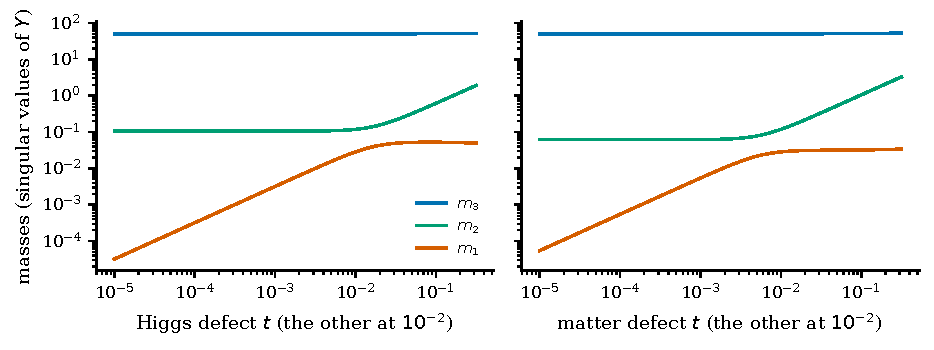
\includegraphics[width=\linewidth]{figures/fig_joint}
\caption{The joint law (Theorem~\ref{thm:joint}): two defects and three masses, an illustrative recomputation from the
theorem's formulas (not an arc's output). In the twisted frame, with a null Higgs and a null matter perturbed by
defects of scale $t$ (left: the Higgs; right: the matter; the other side's defect fixed at $10^{-2}$), the heaviest mass
stays, the middle mass reads the larger defect's term, and the lightest, bilinear in the two defects, falls linearly in
the varied one until it meets the other. Exact identities over $M_2(\C)\times M_2(\C)$ at one $\tau$; no data.}
\label{fig:fig_joint}
\end{figure}

\reading{The coupling's shape is two defects and a pairing. Each defect measures how far a field sits from the null cone;
a null vector is a field, or a pairing, that sits exactly on it. What the grammar fixes is this shape. Where the
fields sit is the choice of a world.}

\subsection{The period phase: the bridge to the motion}\label{sec:phase}

The couplings so far hold at one point of the modular surface. The threads of Section~\ref{sec:weave} are closed paths
through it, and the matter's defect $D$ of Proposition~\ref{prop:norm} is a function along each. How $D$ transforms under
the moves decides how an amplitude built from it can be averaged over a thread.

\begin{lemma}[Automorphy of the defect]\label{lem:automorphy}
The defect $D$ has weight $-1$ and the multiplier $\chi$ of $\eta^6$: for $g=\begin{psmallmatrix}a&b\\c&d\end{psmallmatrix}$
in the modular group, $D(g\tau)=\chi(g)(c\tau+d)^{-1}D(\tau)$, with $\chi(\tau\mapsto\tau+1)=\chi(\tau\mapsto-1/\tau)=i$. Hence $\chi(L)=i$ and
$\chi(R)=-i$ for the two letters of the grammar.
\end{lemma}
\begin{proof}
Write $D=-\theta_3^4h(\lambda)/(4\pi\eta^6)$ with $\lambda=\theta_2^4/\theta_3^4$ and
$h(\lambda)=\lambda\log|\lambda|+(1-\lambda)\log|1-\lambda|$ (the closed form checked in B1657). Under $\tau\mapsto\tau+1$,
$\theta_3\leftrightarrow\theta_4$ and $\theta_2\mapsto e^{i\pi/4}\theta_2$, so $\lambda\mapsto\lambda/(\lambda-1)$ and
$\theta_3^4\mapsto\theta_4^4=\theta_3^4(1-\lambda)$; a short computation gives $h(\lambda/(\lambda-1))=-h(\lambda)/(1-\lambda)$, and
$\eta^6\mapsto i\eta^6$. Hence $D(\tau+1)=iD(\tau)$. Under $\tau\mapsto-1/\tau$, $\theta_3\mapsto\sqrt{-i\tau}\,\theta_3$ and
$\theta_2\leftrightarrow\theta_4$ with the same factor, so $\lambda\mapsto1-\lambda$, $\theta_3^4\mapsto-\tau^2\theta_3^4$,
$h(1-\lambda)=h(\lambda)$, and $\eta^6\mapsto(-i\tau)^3\eta^6=i\tau^3\eta^6$. Hence $D(-1/\tau)=i\,\tau^{-1}D(\tau)$. Both sides of the
law compose by the cocycle rule, and the two maps generate the modular group, so the law holds on the group. The letters
follow from $L:\tau\mapsto\tau+1$ and $R=S_0L^{-1}S_0^{-1}$ (Appendix~\ref{app:hand}).
\end{proof}
\noindent\emph{Remark.} $D$ is real-analytic, not holomorphic, because of $\log|\cdot|$; the law is nonetheless exact. The
record also checks it numerically at $L$, $R$, $S_0$ and $L^{-1}R$, to $10^{-30}$.

\begin{theorem}[The period phase]\label{thm:phase}
Along a thread, let $z(s)$ be the geodesic in the upper half-plane, with $s$ its arclength, and let
$\psi(s)=D(z(s))\,(dz/ds)^{-1/2}$ be the \emph{amplitude}. Then after one period the amplitude returns multiplied by
\[
  \psi(s+\ell)=i^{\,\#L-\#R}\,\psi(s),
\]
the exponent counting the letters of the thread's word $\gamma$. Consequently a coherent average of $\psi$ over a thread survives
only if $\#L\equiv\#R\pmod 4$.
\end{theorem}
\begin{proof}[Proof sketch]
Along a closed geodesic the period is the hyperbolic element $\gamma=\begin{psmallmatrix}a&b\\c&d\end{psmallmatrix}$ of the
thread's word, with $z(s+\ell)=\gamma z(s)$. The derivative $dz/ds$ transforms by $(cz+d)^{-2}$ and $D$ by
$\chi(\gamma)(cz+d)^{-1}$ (Lemma~\ref{lem:automorphy}). Let $r(s)$ be the ratio of the continuation of $(dz/ds)^{-1/2}$
from $s$ to $s+\ell$ to its value at $s$. Then $r^2=(cz+d)^2$. Since $cz+d$ has no zero on $\Hb$ and $r$ is continuous,
$r=\epsilon\,(cz+d)$ with one sign $\epsilon$ for all $s$. As $s\to-\infty$, both $z(s)$ and $z(s+\ell)$ tend to the
repelling fixed point $x$ of $\gamma$ and the two tangent directions agree; for $s$ negative enough the argument of $dz/ds$
varies by less than $\pi$ along $[s,s+\ell]$, so the continued square root takes the principal branch of a ratio that
tends to a positive number (a power of
the ratio of the two heights), while $cz+d\to cx+d$. This is an eigenvalue of $\gamma$, positive because a word in $L$ and
$R$ has positive trace. Hence $\epsilon=+1$, $\psi(s+\ell)=\chi(\gamma)\psi(s)$, and
$\chi(\gamma)=\chi(L)^{\#L}\chi(R)^{\#R}=i^{\#L-\#R}$ because $\chi$ is a character. Census law~\ref{cl:phase} (B1666) checks
this numerically.
\end{proof}
\noindent\emph{Scope.} Exact for every thread, by Lemma~\ref{lem:automorphy} and the argument above. It concerns
$D$ alone, not the physical amplitude, which also needs the Higgs's own transformation (the determinant and the pairing)
that B1656's frame leaves free.

\begin{figure}[t]
\centering
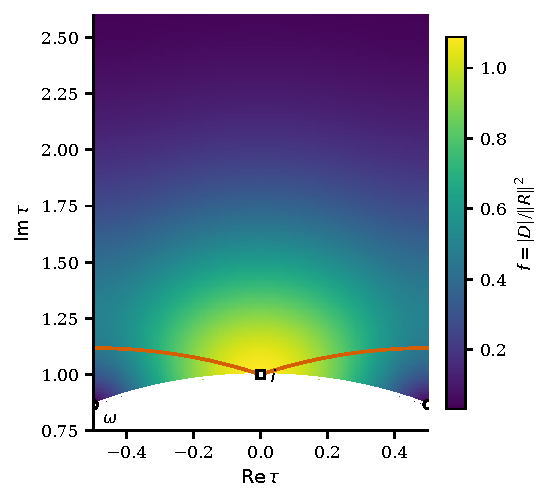
\includegraphics[width=0.55\linewidth]{figures/fig_defect}
\caption{The matter's defect relative to its norm, $f=|D|/\|\rho\|^2$, on the fundamental domain. It is modular-invariant
(Lemma~\ref{lem:automorphy}), vanishes at $\omega$ and toward the cusp, and peaks near $i$. The root $LR$'s closed geodesic,
reduced to the domain, passes through $i$. Computed with the sealed instrument's $f$ (B1663).}\label{fig:defect}
\end{figure}

\begin{censuslaw}[Period phase over the threads; B1666]\label{cl:phase}
On all $30\,674$ threads with trace at most $600$ the least-squares phase over two consecutive periods,
$\sum g(s+\ell)\overline{g(s)}/\sum|g|^2$, equals $i^{\#L-\#R}$ with error at most $1.1\cdot10^{-7}$. The phase is $1$ on
$0.2508$ of the threads, as the four values of the character predict. The ratio includes the square root's branch, so
the census checks numerically the branch sign $+1$ that Theorem~\ref{thm:phase} proves for every thread.
\end{censuslaw}
\noindent\emph{Scope.} A census to trace $600$; no statement for longer threads. It is a sealed test (preregistered, run
once), and the earlier gates that failed at the zeros of $D$ (B1664, B1665) are disclosed in Section~\ref{sec:methods}.

\paragraph{What the bridge shows.}
Two companion readings from the same sealed arc, both scoreboards (the data of B1664 and B1665 were seen, so they are not
blind), are developed in Section~\ref{sec:boundary}. Averaged trace by trace, the threads' average of the defect
$f=|D|/\|\rho\|^2$ approaches the constant mode of the modular surface, $0.31500491$, as the equidistribution of closed
geodesics predicts~\cite{Duke1988,Sarnak1982}; and the amplitude, unlike the size, has no constant wave: its
coherence falls with length. The first is expected, the second is the content. Neither fixes a value of the Standard Model.

\section{A chiral index $\pm3$, given its inputs}\label{sec:three}

\paragraph{The question.}
The couplings of Section~\ref{sec:couplings} treat the triplet as a representation. A generation, in the physical
sense, is a \emph{count} of chiral fermions, which is an index. We ask when the grammar's triplet becomes such a count
and what must be assumed. The answer is conditional on stated inputs, and it is not an index of a thread. On any cusped
three-manifold or cover every twisted Euler characteristic vanishes (B1604; Boundary result~\ref{bd:noindex}), so no flat-module count on a single thread is a chiral index. The count lives on the fibre
family, as follows. The record is cited by arc~\cite{OriginAxiomRepo}.

\paragraph{The setting.}
The weave's surface is $M_{1,2}$, the moduli of a torus with two marked points, taken as the weave's surface by a reading made
within the program, of which the record verifies only the Euler characteristic (B1624). Its fibre loops, the point-pushes, are the inner automorphisms,
and the weave's moves lift to the matter by the lift that agrees with the ruled moves (B1641). That lift is the record's:
$\mathrm{conj}(a)$ and $\mathrm{conj}(b)$ act on the triplet by the parity signs and the commutator loop by $-1$, which is
$\Delta^4$ of the moves. The geometric lift, trivial on cohomology, differs from it by that central sign at $\Delta^4$.

\paragraph{The inputs.}
\begin{itemize}
\item \textbf{The triplet postulate} (Table~\ref{tab:inputs}): the left-handed matter lives in the triplet $T$ and the mass
  tensor couples it. A tagged working postulate, in the record the subspace named $\Lambda$ (renamed here to avoid the
  cosmological constant). What would discharge it: an even-dimensional object with a non-flat bundle whose index is the
  count.
\item \textbf{One cusp unit}: the cusp contributes $n$ units of the end datum, with $n=\pm1$ when one unit is taken.
  A tagged working postulate. What would discharge it: an end mechanism at the cusp.
\item \textbf{The extreme boundary domain}: the subspace $\Lambda_+$ of the critical coefficients at the cusp is taken to be
  $0$ or the whole module $L_6$. Other admissible domains give $\pm1$ (below). What would discharge it: a rule that selects
  the domain.
\end{itemize}
The setting, $M_{1,2}$ as the weave's surface with the lift that agrees with the ruled moves, is a reading verified only
in part, and we list it with the inputs.
None is derived in the record: the first is a postulate, the second a normalisation at an end the grammar does not fix,
the third a choice of domain. All are priced in the inputs table (Table~\ref{tab:inputs}). The ``$3$'' is the dimension
of the postulated triplet, read through the extreme domain; it is not a derived count of generations.

\begin{theorem}[The index $\pm3$; T6]\label{thm:index}
Given the triplet postulate and $n$ units at the cusp, on $M_{1,2}$ with the weave's lifts, the four-dimensional index
is $n(|\Lambda_+|-3)$, where $|\Lambda_+|$ is the dimension of the chosen subspace $\Lambda_+$ of the critical coefficients at the cusp. For
$\Lambda_+=0$ the index is $+3,0,-3$ for $n=-1,0,1$; for the two-dimensional piece $V_2$ of the six-dimensional module it
is $+1,0,-1$ and for $V_4$ it is $-1,0,+1$; and for the full module $L_6$ it is $-3,0,+3$. With one cusp unit, $n=\pm1$,
a non-zero (chiral) index is therefore $\pm3$ for $\Lambda_+=0$ or $\Lambda_+=L_6$.
\end{theorem}
\begin{proof}[Proof sketch]
The six-dimensional module $L_6$ is a representation of the metaplectic cover $\mathrm{Mp}_2(\Z)$ with exponents
$(1,1,3,5,7,7)/8$ and commutant of dimension $2$ (braid relation exact). It splits as $V_2\oplus V_4$, two non-isomorphic
irreducibles, so no three-dimensional constituent exists. The characters $\chi_1$ of the pieces and of $L_6$ vanish and
$\chi_{3/2}(\rho_T)=0=\chi_{1/2}(\bar\rho_T)$, so weight one is allowed, and the dimension formula for vector-valued modular forms
(as used in B1632) gives the fibre's contribution; the index is $n$ times it. The table is verified in both identifications of the module.
See B1641.
\end{proof}
\noindent\emph{Scope.} Verified for the module and the lifts named; the setting, $M_{1,2}$ as the weave's surface, is a
reading, and whether the lifts cohere over the whole of $\mathrm{Aut}^+(F_2)$ is open. The theorem is conditional on both inputs, and \emph{conditional} is the word: with $n=0$, or without the triplet
postulate, there is no count. B1641 also finds, by its sealed read-out, that the hand is \emph{not} the puncture
condition's orientation at the representation level: neither $\rho_T$ nor its conjugate is a sub or quotient of $L_6$. It
makes no claim about the hand (Section~\ref{sec:selection}).

\paragraph{The end radius, and what fixes it.}
Proposition~\ref{prop:norm} introduced the end radius $L=\log(1/\epsilon)$ of a disc removed at the puncture. B1656's
channel norm is the regularised norm with $2\pi L$ subtracted, and the first generation's lift $D/(2\pi L)$ depends on
it. In the flat metric a complete cusp has no boundary on which to impose a condition, and $L$ behaves as a free scale
(B1654). In the fibre's own complete hyperbolic metric, the uniformisation of the punctured torus, the puncture is a
hyperbolic cusp. A hyperbolic cusp has canonical neighbourhoods: the maximal embedded horoball, and the horocycle of
length $2$, which is embedded by Shimizu's lemma. Each fixes $L$ as a function of $\tau$ alone.

\begin{censuslaw}[the canonical cusp; B1667]\label{cl:cusp}
On a grid over the fundamental domain up to $\operatorname{Im}\tau=4$ ($54$ points), the maximal cusp gives
$L_{\max}\in[0.643,0.691]$ and the horocycle of length $2$ gives $L_2\in[2.29,2.78]$. At $\tau=e^{i\pi/3}$ both equal a
closed form from the periods of $\eta^4$: the punctured hexagonal torus is $\Hb/\SL(2,\Z)'$, freely generated by $LR$ and
$RL$. Under either canonical cut, the first generation's lift, computed with the exact channel norms outside the
horoball, is a function of $\tau$ alone. It is $0.03$ to $0.41$ in the bulk, has a simple zero at $\omega$, and falls like
$e^{-2.6\operatorname{Im}\tau}$ toward the cusp of moduli.
\end{censuslaw}

\noindent The end therefore supplies no hierarchy: a large $L$, which the bulk hierarchy $m_1/m_3\approx0.15/L$ would
need, is a cut far inside every canonical horoball, at a scale the fibre's geometry does not supply. The end datum is a
discrete choice between canonical horocycles, not a continuum, and a small first generation becomes a statement about
$\tau$. The computation is a census over the grid, informed by points seen before its seal. It does not say which
canonical horocycle, if either, is the physical end.

\paragraph{Does the symmetry fix the domain?}
If the domain must be preserved by the moves, the freedom drops from a continuum to the invariant subspaces of $L_6$. By
the proof above, $L_6=V_2\oplus V_4$ with $V_2$ and $V_4$ inequivalent and irreducible; the group the moves generate on
$L_6$ is the binary octahedral group $2O$, of order $48$ (B1606). So the invariant domains are $0,V_2,V_4,L_6$, and the
index is $\pm3$ or $\pm1$ (the record's kept indices $-3,-1,+1,+3$, B1606). The symmetry therefore
restricts the count but does not force three: an invariant domain of dimension three, which would leave only $-3,0,+3$,
does not exist, because $L_6$ has no three-dimensional constituent. The extreme domain remains a choice. Whether a
finite-distance model of the puncture, whose index is also $\dim\Lambda-3$, carries the same module is open.

\reading{The triplet is a representation until something counts it. What counts it is not in the grammar: one postulate
says where the matter lives, one unit says how many times the end is taken, and one choice says which boundary domain is
kept. A chiral three is thereby a question about the cusp's end, not a consequence of the moves.}

\section{The boundary}\label{sec:boundary}

\paragraph{The question.}
The structure of the previous sections holds on the inputs of Table~\ref{tab:inputs}, and it fixes no number. The principle asks for more than structure: it would have to single
out a world. This section asks how far the same structure reaches toward the Standard Model's flavour numbers, and
where it stops. We answer with results of one kind, each stated with its frame and its grade: what the weave's
symmetry, its clock, its frames and its motion do \emph{not} fix. The results are labelled N1--N7. Four of them (N4--N7) are sealed negatives, a compiled verdict, or sealed
scoreboards. The one-Higgs census (N5) tests a model of the program's own (one Higgs, $\tau=\omega$, eighteen flat lines),
so it locates the boundary of the program and not of the grammar. All of them are kept in the paper, because a boundary located only by success would not be located. The
program's arcs are cited by number (B1604 and so on) as the record, not as papers~\cite{OriginAxiomRepo}. No result
below is a value of the Standard Model (0 of 19).

\paragraph{The spine.}
A law of invariance fixes an orbit, not a point of it: a selector that commutes with a group acting on the possible
numbers cannot choose among the points of one orbit (the record's orbit-to-point gap, B990, stated there for orbits of
pairs of $27$s).
At a point of the fibre the residue coupling has rank one and the coupling has rank at most two for every flat line
(B1653); at the symmetric point $\tau=\omega$ the Higgs's symmetric vacua give masses $(1,1,0)$, a rank-one coupling, or a
hierarchy set by the two defects (B1657), and the isotropic vacua carry no hierarchy of their own. Hence whatever chooses the numbers is not given by the
symmetry alone, although it acts at one. N1--N4 below are the symmetry side of this statement; N5--N7 are the
quantitative side, on the matter and the motion.

\subsection{No index on a thread}

\begin{lemma}[N1; B1604]\label{bd:noindex}
Let $N$ be the interior of a compact $3$-manifold with torus boundary (a cusped hyperbolic $3$-manifold, or a finite
cover of one), and let $E$ be any flat module. Then
\[
  \chi(N;E)=\chi(N,\partial N;E)=\operatorname{rank}(E)\,\chi(N)=0,
\]
because $\chi(N)=\tfrac12\chi(\partial N)=0$: the double $N\cup_{\partial N}N$ is a closed odd-dimensional manifold, so
$0=2\chi(N)-\chi(\partial N)$, and $\chi(\partial N)=0$ for a torus. By Poincar\'e--Lefschetz duality $h^2(N;E)=\dim H^1(N,\partial N;E^*)$ and
$h^3(N;E)=0$. The class index $I(E)=n(E)-n(E^*)$, where $n(E)$ is the dimension of the interior cohomology, the image of
$H^1(N,\partial N;E)\to H^1(N;E)$, and $n(E^*)$ equals, by duality, the interior dimension of $E$ in degree two, is therefore not an Euler characteristic, and no
index theorem of Euler type computes it.
\end{lemma}

\emph{Scope.} This is standard topology (the vanishing of $\chi$ on odd-dimensional manifolds, and duality) applied to
the record's class index; the application is the arc's. The consequence is the one we use: a generation count obtained
as a flat-module index on a thread, or on a cover of one, is not given by an Euler-type index theorem; this argument does not exclude other index constructions. The
record also finds, by computation on the modules it checked, that $I(\Lambda^2E)$ is not a function of $I(E)$ (B1603). A
physical count needs an even-dimensional object with a non-flat bundle, or else ``a generation'' means a sector
selected by a character, which is a selection. This is why the chiral three of Section~\ref{sec:three} is stated with
three inputs and a reading, and not as a consequence of the thread alone.

\subsection{Residual symmetries against the data}

\begin{theorem}[N2; B1620, B1625]\label{bd:reducesnone}
Let $G$ be the weave's group (the lifts of $L$ and $R$ on $V=T\oplus\bar T$; order $96$, faithful and irreducible on the
triplet $T$). Take every subgroup $H\le G$ ($68$ subgroups in $26$ classes) as the residual symmetry of one sector, none
chosen.
\begin{enumerate}
\item A sector has three distinct masses exactly when $T|_H$ is a sum of three characters, that is when $H$ is abelian ($57$
  of the $68$), and every such residual leaves the masses free.
\item For every ordered pair of such residuals the family of mixing matrices has dimension $0,1,2,3$ or $4$ (the rank of
  the map to the nine $|V_{ij}|^2$ and the Jarlskog invariant), and no family of dimension below $4$ reaches the CKM
  matrix at $3\sigma$.
\item This holds with the mass term in $\bar T\otimes T$, in $T\otimes T$ and in $\mathrm{Sym}^2T$ (with $57$, $24$ and
  $16$ viable subgroups), and in every frame on record where the inner automorphisms act.
\end{enumerate}
\end{theorem}

\emph{Scope.} Proved by exhaustive computation over the subgroups and the three tensors; the block test used for the
CKM bound is necessary and sample-free, while the reach of the PMNS matrix is decided by a fit (and was regraded with
a strict predicate in B1625, the minimum unchanged). The statement is scoped, as the record scopes it, to the frames
where the inner automorphisms act; on the ruled branch the count is a lower bound under the modular-flavour ansatz. For
couplings in the modulus $\tau$ alone, the inner automorphisms generate an abelian group of order four that splits $T$
into three lines with distinct characters, so every mixing is a permutation (B1620). The statement is of a known kind. Scans
of the residual symmetries of finite groups find, in the settings they consider, quark mixing at leading order that gives
the Cabibbo angle and not the full CKM matrix~\cite{HolthausenLim2013,YaoDing2015}. The result here is the same answer for
this particular group, computed on all its subgroups; we are not aware of a published discrete-flavour model that
reduces the thirteen by a definite number~\cite{Feruglio2019,NovichkovPenedoPetcov2021}.\footnote{A fourth boundary statement, a count of the
parameters that one-modulus modular fits need (B1637), is not stated here. Its near-cusp fits were artifacts of the
evaluator's precision, and its re-run on an accurate evaluator is owed.}

\subsection{The clock stays in the grading}

\begin{theorem}[N3; B1621, B1633]\label{bd:clock}
Let the clock be the parity class $(A_n,B_n)$ modulo $2$ of the rule's fixed-point word, acting on $T$ as conjugation
by the word's prefix, which is $\mathrm{diag}(\chi_p)$ on $T$.
\begin{enumerate}
\item The clock's matrices span exactly the diagonal algebra. Every coupling that reads the clock is diagonal in the
  parity lines under every tensor: it splits masses and never mixes, and its invariant mean on $T$ is zero.
\item The tick $\sigma^2=LR$ acts on $T$ with eigenvalues $\{1,\omega,\omega^2\}$ and cycles the parity lines. Its
  operator mean is the rank-one democratic matrix, which does not commute with the clock, and its means on the clock's
  forms give three equal masses under all three tensors.
\item The averaged word coupling is a scalar on $T$ (B1633).
\end{enumerate}
\end{theorem}

\emph{Scope.} Exact up to floating point, with the word taken to $F_{30}$. The democratic matrix is classical; the
statement that it is a mean and not a commutant leaves the earlier refutation of $\mathbb Z/3$-forced democracy untouched.
The consequence is that the principle's own data (its clock and its tick) fix no number: they supply a grading and a
scalar.

\subsection{The frame tribunal}

The same computation gave different answers in different frames: the first-generation zero holds in one and dies in
another, and ``the Higgs in $M$'' is the electroweak Higgs in one frame and a flavon in another. A value can be
derived only along a chain with no hidden choice, and the frame is the first link of every chain, so the frames were
judged before further numbers were chased.

\begin{verdict}[N4; B1652]\label{bd:tribunal}
Take the frames on record (F1, the fibre at one $\tau$; F2, the surface frame with $\tau$ integrated; F3, an E$_8$
frame studied within the program; F4, the thread frame) and the eight demands D1--D8: the moves act as symmetries; the chiral
three; an anomaly-free hypercharge; an electroweak Higgs that couples the matter; a possible hierarchy; no free number
beyond the tagged postulates; CP violation possible; the scale and gravity. Then no frame on record is shown to
satisfy the demands on its own. The parent that would satisfy all of them is a seven-clause specification, and it is a
conjecture.
\end{verdict}

\emph{Scope.} A compiled verdict on the record's evidence of 2026-10-14, with each cell graded and cited. ``Shown''
means shown by a computation reproduced in the record; cells resting on an unreproduced computation are read and not
built on, and the
verdict needs only the verified failures and the untested cells. Representative cells, not the table:
F1 holds the chiral three given the triplet postulate and allows CP violation, but its hierarchy needs a free number
per sector and its D1 holds only given a vacuum that no dynamics on record selects; F2 holds the moves but needs a
source from outside the weave for the three and forbids CP violation; F3 holds the moves only by a supplied completion
that, on its flat background, loses the weak roots and the hypercharge, and its physical index is not computed. A
further candidate, formed inside the program, was refuted by the record (it fails D2 and D4 on the data) and is not
counted. The scope note on F3 applies: the table is evidence that no exhibited frame discharges every demand,
not that every frame fails.

\subsection{One Higgs against the data: a scoreboard}

\begin{scoreboard}[N5; B1660; negative as sealed]\label{bd:census}
On none of the eighteen admissible lines at the symmetric point $\tau=\omega$, in none of three readings of the up
sector (the same coupling $S$, the coupling $\tilde S=\epsilon\bar S\epsilon^{T}$, and the conjugate $\bar S$), does a single Higgs reproduce the data's five
non-electron mass ratios: no fit was found below the conservative bound $\chi^2=11.07$ (the $95\%$ point of $\chi^2$
with five degrees of freedom; the minimum over the fit's parameters is at most the value at the true point, so the bound
is one-sided and conservative), and the best was $34.40$ (the
conjugate reading on the pair of lines $(p_1,p_2)=(1/9,7/9)$ and $(8/9,2/9)$, with $w=p_1\tau-p_2$).
\end{scoreboard}

\emph{Scope.} A scoreboard, not a blind test: the data~\cite{HuangZhou2021} were seen. The census is for the canonical
end condition and the twisted frame of Section~\ref{sec:couplings}, at $\tau=\omega$, and the search was shown to recover
planted worlds in the data's regime. The end radius was a free parameter of the fit, over a domain
($2\pi\mathcal E+c_s>0.5$ in every channel, unbounded above) that contains both canonical radii at $\omega$ (Census
law~\ref{cl:cusp}: $0.692$ and $2.786$), so the canonical radii are among the values the fit could take. Its starts had
$\mathcal E\ge2.5$, and the lift with the exact norms outside a horoball differs from B1654's form by 17 to 25 per cent
(B1667). The end radius is a free parameter of the search, so the best value found bounds the best fit from above only. The census therefore does not by itself certify the result at a fixed radius, such as the canonical cuts of Census law~\ref{cl:cusp}. The misses are the two middle ratios, $m_s/m_b$ too large and $m_\mu/m_\tau$ too
small. The data put $(m_\mu/m_\tau)/(m_s/m_b)$ at $3.14$ ($2.9$ to $3.4$ within the strange-quark mass's uncertainty
alone)~\cite{HuangZhou2021}, against $0.63$--$1.75$ at the best points of the census
(Figure~\ref{fig:census}); the up quarks' $m_1/m_3$ is met. The Georgi--Jarlskog relation between the down quarks' and
the leptons' middle masses~\cite{GeorgiJarlskog1979} is context, not a claim.

Two post-seal explorations bound what the negative means, and both are labelled as explorations. First, there is no
ceiling: with no other target, the ratio $(m_\mu/m_\tau)/(m_s/m_b)$ reaches between $9$ and $34$ over every Higgs and
every end radius on four lines, so the misfit is a joint conflict among the five targets and not a bound on one of them.
Second, without the up quarks the down and lepton targets fit exactly. A second Higgs for the up quarks therefore makes
the ratios fittable, which is why it needs a blind test and not a further scoreboard.

\begin{figure}[t]
\centering
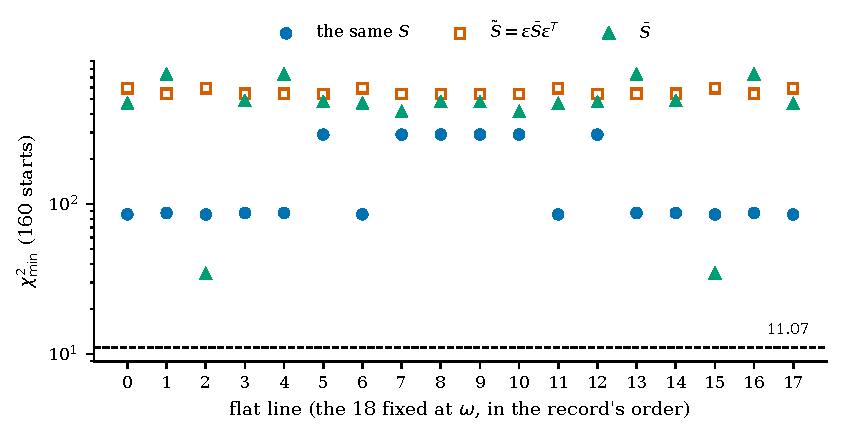
\includegraphics[width=\linewidth]{figures/fig_census}
\caption{B1660's scoreboard. The best $\chi^2$ (160 starts) on each of the eighteen admissible lines in each of three
readings of the up sector, against the conservative bound $11.07$. Scope: one Higgs at
$\tau=\omega$ on the admissible lines, the data seen; a scoreboard, not a ceiling, and not a statement about two Higgs
fields.}\label{fig:census}
\end{figure}

\subsection{The pull-back's strength}

The grammar's states move: a walk of steps and their pull-backs escapes at a positive rate whatever the pull-back's
strength (for the symmetric walk by Kesten~\cite{Kesten1959} and Furstenberg~\cite{Furstenberg1963}; for the other weights
by the same theorem of Furstenberg, as the support generates $\SL(2,\Z)$; the rates are measured here). We call the pull-back's weight $p$ (the probability of choosing a pull-back
at each step). The question is which quantities the weight $p$ sets.

\begin{censuslaw}[N6; B1663; negative as sealed]\label{bd:strength}
For $p=0,0.1,\dots,0.5$ the walk on $L,R,L^{-1},R^{-1}$ (equal weights within each pair) has the following behavior.
\begin{enumerate}
\item The probability that the end lies on the positive side falls from $1.000$ at $p=0$ to $0.531\pm0.028$ at
  $p=\tfrac12$ ($\tfrac12$ exactly there, by the mirror).
\item The escape rate falls from $0.3959\pm0.0004$ per step at $p=0$ to $0.1007\pm0.0005$ at $p=\tfrac12$. The escape rate
  is $(1/n)\log\|X_n\|_F$ at the first $n$ at which an entry of the walk's product $X_n$ exceeds $10^{60}$ (or at
  $n=40\,000$), an estimate of the top Lyapunov exponent, which is half the hyperbolic drift of $d(i,X_n i)$. This
  first-passage estimator differs from a fixed-length estimate by about $0.1\%$ at $p=0$ (low) and about $2\%$ at
  $p=\tfrac12$ (high): the fixed-length estimate gives $0.3964\pm0.0001$ and
  $0.0987\pm0.0002$ (\texttt{checks/lyapunov\_fixed.py}; B1662 reports $0.0992$ at $p=\tfrac12$).
\item The motion's averaged defect $\langle f\rangle$ is $0.5157\pm0.0012$ at $p=0$ and $0.5178\pm0.0013$ at
  $p=\tfrac12$; over all six values of $p$ it varies by $0.0028$. The preregistered prediction that it would differ by
  more than five standard errors failed.
\end{enumerate}
\end{censuslaw}

\emph{Scope.} The statement is for $L$, $R$ and their inverses with equal weights within each pair, with resolution about
$0.009$: a mild dependence of that size is not excluded. The averaged defect is a definite number, $0.517$, the forward
motion's; it differs from $0.31500491$, the average of $f$ over the modular surface, which is the value along a typical geodesic
(the \emph{typical motion's} value), and no dictionary attaches it to a mass. The strength $p$
sets the side and the speed. It does not set the defect, so the pull-back adds no number to the sizes.

A post-seal exploration, labelled, bears on why. The continued-fraction digits of the limit follow the geometric law
$2^{-k}$ at $p=0$ and at $p=\tfrac12$ alike (frequencies $0.502,0.248,0.123,0.064$ and $0.504,0.253,0.121,0.060$ for the
digits $1$ to $4$, on $24\,000$ digits each), against the Gauss--Kuzmin law $0.415,0.170,0.093,0.059$ of a typical point.
At $p=0$ the geometric law is exact and classical: the steps are fair independent letters, the digits are their run
lengths, and the limit's law is Minkowski's measure $d{?}(x)$, which is singular~\cite{Denjoy1938,Salem1943}. The $p=0$
reading is therefore a control. At $p=\tfrac12$ the same law is a reading of $24\,000$ digits and not a proof. For
$p>0$ the steps generate the group, and the exit law of a finitely supported generating walk is singular: for
$\SL(2,\Z)$ by~\cite{GuivarchLeJan1993}, and for nonuniform lattices in general by~\cite{GadreMaherTiozzo2015}. We use
neither statement beyond that scope.

\begin{figure}[t]
\centering
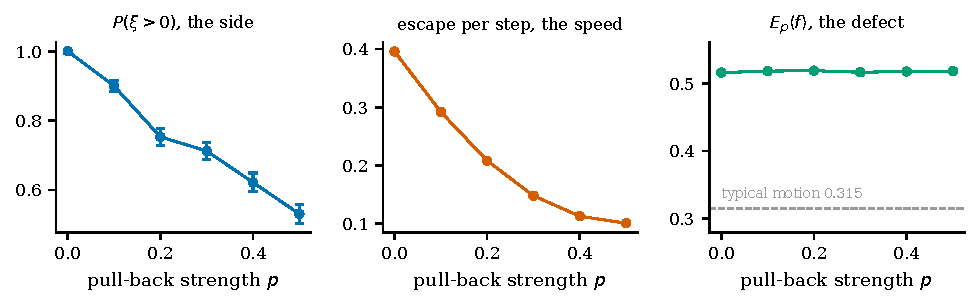
\includegraphics[width=\linewidth]{figures/fig_pullback}
\caption{B1663. (a) The side $P(\xi>0)$, (b) the escape rate and (c) the averaged defect $\langle f\rangle$ against the
pull-back weight $p$, with the typical motion's $0.31500491$ marked. Scope: the walk on $L^{\pm1},R^{\pm1}$ with equal
weights within each pair; the flat panel (c) is the negative result, and its resolution is about $0.009$.}\label{fig:pullback}
\end{figure}

\subsection{The layers}

The weave has two sides, the sum over closed geodesics (the threads) and the spectrum of the modular surface (the waves).
We asked what the threads' layers do on the program's own quantity, the matter's defect $D$ with $f=|D|/\|\rho\|^2$. The
sequence of arcs is part of the result. B1664 and B1665 were sealed and failed their own gate at the two zeros of $D$
(Section~\ref{sec:methods}); both are recorded as inconclusive. B1666 re-sealed the test with an estimator that no
zero can spoil; its cells hold, and it is a sealed scoreboard, because the read-outs of the first two were seen.

The period phase is Theorem~\ref{thm:phase}, which holds for every thread (checked to trace $600$,
Census law~\ref{cl:phase}): a coherent average of the amplitude survives only on the quarter of threads with
$\#L\equiv\#R\pmod4$. The layers then give the following.

\begin{scoreboard}[N7; B1664--B1666]\label{bd:layers}
To trace $600$, and on the threads of that range:
\begin{enumerate}
\item the layer averages of $f$ by trace approach the typical motion's $0.31500491$ (the top quarter of the traces, $451$ to
  $600$, gives $0.3144$, against $0.3692$ for traces at most $20$), with the distance falling as
  $t^{-0.51\pm0.05}$;
\item the phase-one coherence of the amplitude falls with length, with slope $-0.269\pm0.083$. The \emph{coherence} of a
  thread is $\bigl|\int\psi\,ds\bigr|/\int|\psi|\,ds$ over one period, and the phase-one threads are those whose period
  phase is $1$. The slope is $3.2$ standard errors from $0$ and $2.8$ from the random-phase value $-\tfrac12$, the error being
  an ordinary least-squares error over threads treated as independent;
\item the normalised coherence of the cusp family $L^{4m+1}R$, after a first drop, climbs toward one ($0.637$ at $LR$, then
  $0.285,0.717,0.861,0.919,0.948,\dots,0.99994$), and the most coherent phase-one thread is the longest of the family.
  The root $LR$ is not singled out. This is a read-out with no criterion, and the size of the coherent amplitude is not
  compared.
\end{enumerate}
\end{scoreboard}

\emph{Scope.} Item~1 is the trace formula's constant mode on the program's own quantity, expected from the
equidistribution of closed geodesics on the modular surface and of their discriminant layers~\cite{Duke1988,Sarnak1982}, with cycle integrals as in~\cite{KatokSarnak1993}; it is a check of the weave side against
the wave side, not a new equidistribution theorem. The law of the phase is a sealed identity; items~1--3 are a
scoreboard (the earlier read-outs were seen). What it does not show: the physical amplitude (this is $D$ alone, and the
physical amplitude needs the Higgs's own law), any Standard Model value, or the rate of approach as a law. The approach to the constant mode is a property of bounded
quantities such as $f$; it is not claimed for quantities that grow at the cusp.

\begin{figure}[t]
\centering
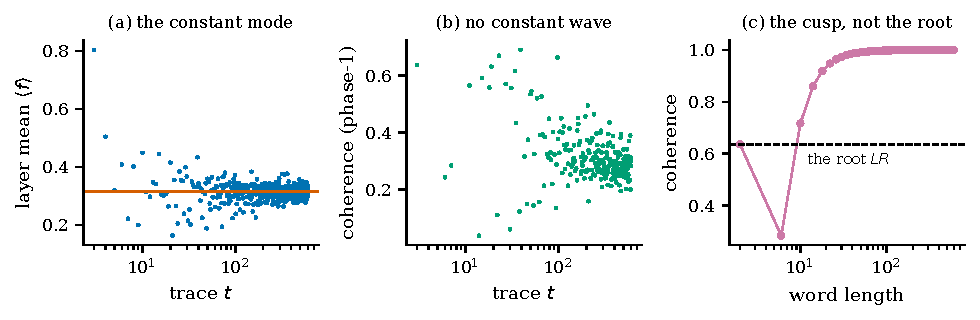
\includegraphics[width=\linewidth]{figures/fig_layers}
\caption{B1666. (a) The layer averages of $f$ against the trace $t$, approaching the constant $0.31500491$. (b) The
layer mean of the phase-one coherence against the trace $t$. (c) The cusp family $L^{4m+1}R$ against word length, with
the root $LR$ marked. Scope: traces at
most $600$, $30\,674$ threads, and the matter's defect $D$ alone; a scoreboard.}\label{fig:layers}
\end{figure}

\reading{The boundary has a shape. What the weave's symmetry, its clock and its frames fix is the structure and none of
the numbers, and each attempt to let a motion choose the numbers returns a constant: the pull-back's strength changes
the speed and not the size; the threads' averages return the surface's own constant; and the one place the motion
prefers something (the coherent rule) it prefers the cusp, where the defect vanishes. This is a reading of
Sections~\ref{sec:boundary} and~\ref{sec:selection} together, and it states no result.}

\section{The open problem: selection}\label{sec:selection}

\paragraph{The question.}
Section~\ref{sec:boundary} located what the structure leaves free. Here we list the free ``which'' choices, state the
shape that a principle selecting among them would have to take, and stop. We do not propose such a principle. Every
statement in this section that is not a cited result of an earlier section is a question.

\paragraph{Every ``which'' is free.} Each of the following is supplied, not derived, in every frame on record.
\begin{itemize}
\item The modulus $\tau$: with the Higgs along $\rho$, the record's invariant quartic selects $\tau=\omega$ or runs to the
  cusp. Neither, as a point, carries a hierarchy (B1652); toward the cusp of moduli the first generation's lift falls
  exponentially (B1667). The record's check covers that direction only.
\item The direction of the Higgs in the triplet's space: it is the second-to-third mass matrix (a bijection onto the
  symmetric $2\times2$ matrices), and no constant direction is covariant under the moves (Section~\ref{sec:couplings}).
\item The line, that is the flat hypercharge line of a sector, among the eighteen admissible lines at $\tau=\omega$
  (B1660).
\item The vacuum, and the frame (Verdict~\ref{bd:tribunal}).
\item The side of the end at which the motion settles (B1663): the pull-back's strength sets the probability of the side and the speed, and
  the choice of side is the positivity of the earlier foundation, now read as a choice.
\item The choice of canonical horocycle at the puncture, which fixes the end radius $\mathcal E$ at order one; the choice is
  discrete, and the record does not make it (Census law~\ref{cl:cusp}, B1667).
\end{itemize}
These choices are not counted in the record's price, four axioms and nine irreducible identifications for the whole
chain. No residual symmetry of the weave's group that reduces the count is compatible with the CKM data at $3\sigma$
(Theorem~\ref{bd:reducesnone}).

\paragraph{The shape of a selection principle.}
Two proved statements constrain it. First, an invariant selector fixes an orbit, not a point of it (B990), and the
symmetric points of the modulus carry rank-one couplings or a hierarchy set by data the symmetry does not fix (B1653,
B1657). Symmetry and orbit invariants alone therefore cannot select a point that is not fixed; an invariant dynamics with a
symmetry-breaking vacuum is not excluded. A selection principle must act where the symmetry is broken or at
its fixed points. Second, the clock and the tick supply a grading and a scalar and nothing else (Theorem~\ref{bd:clock}),
and the pull-back's strength supplies a side and a speed but no size (Census law~\ref{bd:strength}). A principle that
takes its input from either is not enough. What would be enough is stated by the demands of the tribunal: a dynamics on
record and run that selects a vacuum, with the completion and the normalisation named among its inputs
(Verdict~\ref{bd:tribunal}).

\paragraph{The measurer inside the weave.}
A measured value is a comparison between a part of the world and a part that keeps a record of it. Two statements bound
what counting the measurer inside the weave can supply. Neither selects anything.

\begin{lemma}[composition]\label{lem:composition}
Let $r(\gamma,\gamma')>0$ be a read-out on pairs of threads that is to be a ratio of measured magnitudes, so that
$r(\gamma,\gamma)=1$ and $r(\gamma,\gamma'')=r(\gamma,\gamma')\,r(\gamma',\gamma'')$. Then
$r(\gamma,\gamma')=f(\gamma)/f(\gamma')$, with $f(\gamma)=r(\gamma,\gamma_0)$ for any fixed thread $\gamma_0$.
\end{lemma}
\begin{proof}
$r(\gamma,\gamma')=r(\gamma,\gamma_0)\,r(\gamma_0,\gamma')$, and $r(\gamma_0,\gamma')=1/r(\gamma',\gamma_0)$.
\end{proof}
\noindent So, for magnitudes read as composing ratios, a measurer among the threads adds one degree of freedom, the unit.
What remains is a function $f$ on the threads, the form of the per-field read-outs (B1668). The lemma says nothing about
what fixes $f$: an interaction among the threads could constrain it, and read-outs that are not scalar ratios are
outside its scope. A pairwise invariant that does not
compose cannot be a ratio of masses: an example is the linking number of two threads as modular
knots~\cite{Ghys2007,DukeImamogluToth2017}. It can stand only for relational data, such as the mixing between two sectors.

\begin{proposition}[no thread keeps a record, B1675]\label{prop:records}
Take the common point, the quaternion representation $\rho_Q$ ($a\mapsto i$, $b\mapsto j$), with coefficients in the
blocks $\mathrm{Sym}^{2k}\rho_Q$ of $\mathfrak{sl}(n)=\bigoplus_{k<n}\mathrm{Sym}^{2k}$. The private states are the kernel
of the restriction $H^1(F_2;\mathrm{Sym}^{2k}\rho_Q)\to H^1$ of the puncture, $z\mapsto z([a,b])$: the classes that the
puncture, a commutator, cannot detect. They are the flat twists of the block's $Q_8$-invariant part, and at rank three
($k=1,2$) they span four dimensions. On them:
\begin{itemize}
\item no thread keeps a non-zero vector, on all $758$ states to word length $12$;
\item the joint action of $L$ and $R$ keeps none either;
\item a single shear can keep one, and so can the involution $P$: at rank three $L$ and $R$ each keep one class, and
  $P$ keeps two (three at rank four).
\end{itemize}
\end{proposition}
\noindent\emph{Proof and scope.} A thread acts on the private states as its own hyperbolic matrix (eigenvalues
$\lambda^{\pm1}$, $\lambda>1$) tensored with a map of finite order, so it has no fixed vector; a shear is unipotent and
has one. The tables at the common point are exact. The proposition concerns fixed vectors. A relation between two
changing parts can persist without either being fixed (if $x\mapsto Ax$ and $\ell\mapsto\ell A^{-1}$, then $\ell x$ is
kept), so it does not exclude a relational record; whether one exists between the private states and a measurer's
states is a question about equivariant maps between them, not computed here. The census over the threads was decided at $60$ digits on $747$ of
the $758$ states, and on the other $11$ at $120$ digits after the run (B1675).

\reading{The motion's facts, as fenced outlook. The layers' normalised coherence climbs toward one along the cusp family, and not at the root $LR$ (Scoreboard~\ref{bd:layers}). Whether that
selects anything depends on the physical amplitude, which this paper does not construct; we leave the question as stated.
Two computations bound the obvious attempts: in the surface frame's twisted units on the least-volume closing threads, and
in the per-field thread frame at every depth computed, no assignment of the charges, the Standard Model's or a null's,
passes the six-ratio mass test, and the hierarchies come out too strong (B1668).}

\reading{The weave and the wave are the two sides of one equation. The Selberg trace formula equates a sum over the
closed geodesics (the threads, by length) with a sum over the spectrum of the modular surface (the waves, by
frequency), plus terms for the identity, the elliptic points and the cusp; the geometric side runs over the conjugacy
classes that the grammar, with the pull-back, makes reachable states. The shape a selection principle would have to take
is one that reads one side through the other. The layers' constant mode (Scoreboard~\ref{bd:layers}) is this equation's
constant term seen on the program's own quantity. That physics lives on this is not shown.}

\section{Methods: how the record is kept}\label{sec:methods}

\paragraph{The question.}
A program that asks what is forced must show what it assumed and must show its errors. This section says how the
record is kept and gives three corrections as examples. The repository holds every script, output and
lock~\cite{OriginAxiomRepo}.

\paragraph{Sealed preregistration.}
A computation that bears on a claim is written as a preregistration before it is run. It has three parts:
\begin{itemize}
\item its cells, each a prediction with a criterion that can fail;
\item a ``seen first'' section: a sweep of the record for prior work, so that no question is asked twice unknowingly,
  and the literature read;
\item a ``disclosed'' section: everything known or explored before sealing, and any reviewing pass.
\end{itemize}
The preregistration and the instrument are hashed and committed. The instrument is then run once. Its output goes into
its own commit, before the commit that holds any read-out. The history shows that order. That the output was not
looked at in between is the authors' statement, which the history cannot show.

Results are graded by the preregistration's rule: a cell that holds, a cell that fails, or a cell that is an identity
and cannot fail (reported apart from the tests). A result computed on data that were seen is a \emph{scoreboard}, and
its statement says so. Explorations after the seal are labelled and kept apart, with their outputs hashed. A later
change to a sealed file is recorded the same day, in a form that the seal check reads.

\paragraph{Parallel lines and reproduction.}
The work is done on several parallel lines, each on its own branch. A result from one line enters the record as an arc only
after it has been reproduced from its statement on the main line, in independently written code where possible.
Results that were read and not re-run are marked so in the record.
All verification described in this paper is internal to the program. None of it is external review.

\paragraph{Three corrections.}
Errors are recorded as classes and instances in a ledger; the classes this paper meets are listed in
Appendix~\ref{app:corrections}. Three instances from the arcs reported here show the checks at work.
\begin{itemize}
\item \textbf{A read-out that outran its computation (B1660).} The first read-out of the one-Higgs census called the
  down--lepton miss an obstruction that a separate up-quark Higgs ``does not touch'', and implied a ceiling on
  $(m_\mu/m_\tau)/(m_s/m_b)$. Two checks after the seal found no ceiling, and an exact fit once the up quarks are
  dropped. The verdict line was corrected before the result entered the record. Two further faults in the findings
  were repaired at the next review: a step that did not follow, and a headline that rounded two misses.
\item \textbf{A gate that failed at the function's zeros (B1664, B1665, B1666).} The gate asked for the period phase on
  every thread, read at one point of each period. The instrument set $D$ to zero above height $50$, and $593$ of the
  $30\,674$ threads began their sampling there, so B1664 was recorded as open. B1665 moved each start to the period's
  lowest point. That point is the corner at $\omega$, where $D$ also vanishes, and the gate failed on $22$ threads. The
  second repair had not been reviewed. B1666 replaced the one-point ratio by a least-squares phase over two consecutive
  periods, which no zero can spoil. Before the seal, a review checked it on about $2900$ threads, including every
  thread of trace at least $560$; the worst error was $1.1\times10^{-7}$, and the gate was set at $10^{-5}$ on that
  measurement. The sealed run met the gate on all $30\,674$ threads. The rule taken from this: a ratio is never read at
  one point of a function with zeros, and every re-seal is reviewed, however small.
\item \textbf{Checks that read the wrong thing (B1654, B1421).} In B1654, four review helpers read the instrument by an
  absolute path outside the repository. The repair made the paths relative and was noted, but not in the form that
  the seal check reads, so the check reported a disclosed repair as an undisclosed change. The note was recast. Separately, the
  full test suite found a lock (B1421) that still asserted an old count of irreducible inputs after the count had
  become $4+9=13$; the smaller suites run at each landing had missed it.
\end{itemize}

\paragraph{What the method does and does not give.}
It gives a record in which every computed statement has a script, a seal and a stated scope, and in which failures are
kept. It does not give external verification. A statement graded ``proved'' here is proved by the program's own
computation or by a cited theorem. The verification package of Appendix~\ref{app:verify} lets a reader repeat the
load-bearing computations.

\section{What the principle forces, and what it leaves}\label{sec:essay}

This section is an essay. Its sentences are marked: those about mathematics are statements of the preceding sections,
and those about meaning are readings.

\paragraph{Structure on stated inputs.}
We started from one sentence, that existence is what remains when cancelling to nothing cannot complete, and read it as
a grammar of records. The mathematics of the paper is what that reading forces. A first closed path that mixes the
records is the figure-eight's monodromy, under four stated inputs (Theorem~\ref{thm:seed}). Across all closed paths at
once the moves permute the records' three parities, for every word, and carry a triplet, proved for every odd-trace word, with
the arithmetic of its common point a census to length eight (Theorem~\ref{thm:triplet}). Up to a stated hand and a power of the eta character, the triplet's
symmetry is the multiplier of a classical family of theta functions (Theorem~\ref{thm:theta}). In the fibre frame and
given the triplet postulate the coupling ansatz has a null vector at every point (Theorem~\ref{thm:isotropy}); the coupling's
determinant factors through two defects and their pairing (Theorem~\ref{thm:joint}); and, given three stated inputs, a
reading of the weave's surface and an index formula from the record, the index is $\pm3$ (Proposition~\ref{thm:index}). Nothing in this list was
put in to make a number come out. Its first two statements, the parities and the triplet at the common point, hold for every thread at once (the triplet for every odd-trace one); the later
statements hold in one frame.

\paragraph{Unforced selection.}
What the same mathematics does not force is any of the choices that would single out a world (Section~\ref{sec:selection}).
We located each: no residual symmetry of the weave's group that reduces the count of flavour parameters is compatible with the CKM data at
$3\sigma$; its clock stays in a grading; no frame on record is shown to satisfy the principle's demands on its own; one Higgs at the symmetric point fits the five
non-electron ratios on none of the admissible lines; and the strength of the pull-back sets a side and a speed and no
size. The contrast is the paper's organising one. The structure holds on stated inputs, and it fixes no number. Which structure we are in is not fixed.

\reading{A principle of existence that is minimal cannot also be a principle of selection, because selection would be an
additional content. That the structure holds on its inputs and the ``which'' is not fixed is what one would expect if existence were
the remainder of cancelling, and a particular world were a reading of that remainder. The same boundary would also appear if the chosen form were not the principle's own, since the
frames on record share the same postulated triplet and read-out. This is an interpretation of the
boundary and not a consequence of it.}

\paragraph{A third kind of link.}
The record sorts its identifications by what stands on their right. Those between two structures get decided, one way
or the other. Those from a structure to a value have not been earned. Conditions of consistency are a third kind, and
the moves' anomaly is one of them (Proposition~\ref{prop:anomaly}). If the moves act on the fermions as a symmetry,
they must act on left- and right-handed quarks alike. That constrains the dictionary without identifying anything,
which is also how the Standard Model's own hypercharges are fixed. It does not fix a value (0 of 19).

\reading{The measurer as part of the weave. Under the paper's own rule the measurer is not a thread chosen by hand.
Either every thread measures every other, or the measurer is shared by all of them.
\begin{itemize}
\item \emph{What it needs.} A measurer needs a record that its own motion keeps. No thread keeps a fixed one, and neither does
  the weave as a whole; only a shear or the mirror does (Proposition~\ref{prop:records}). So a measurer whose record
  is a fixed state could sit only at an end, a cusp of the modulus or the mirror. A record carried by a relation
  between changing parts is not excluded by that proposition, and is open. Pointer states are likewise the states that the
  measuring interaction leaves fixed~\cite{Zurek2003}.
\item \emph{What it buys.} For magnitudes read as composing ratios it buys the unit (Lemma~\ref{lem:composition}); what fixes the
  ratios themselves is not addressed. Read this
  way, the overall scale is the measurer's unit, and the side of positivity is the direction in which its records
  accumulate, the reading of time as correlation with a clock inside the system~\cite{PageWootters1983}. Neither input
  is discharged; each changes from a fact about the world to a convention of the measurer.
\item \emph{The other two versions.} Selecting only where a measurer can exist needs a criterion of its own, and the
  record's criterion, a kept fixed record, holds on no thread; selection of this kind gives windows, not
  values~\cite{Weinberg1987,AgrawalBarrDonoghueSeckel1998}. Demanding that the measurer's record of a parameter be the
  parameter needs a kept record; a fixed one exists only at an end, where the record already prices the end data as a
  choice. At the fibre's canonical end the radius is of order one (Census law~\ref{cl:cusp}).
\end{itemize}
This is an interpretation, and it fixes no number.}

\paragraph{The push-back picture, as a question.}
One picture motivated this program from its start, and we record it as a question. In it, every step of the grammar is
accompanied by its pull-back; the two are never at rest; and the interaction of the steps with their pull-backs, and not
either alone, is what is real. The mathematics that bears on the picture is proved and is separate from it:
\begin{itemize}
\item the walk of steps and pull-backs escapes at a positive rate: for equal weights by the theorems of Kesten and
  Furstenberg, and at the other weights by Furstenberg's theorem, with the values measured (Census law~\ref{bd:strength});
\item a full turn round a balance point of a step and its pull-back carries the sign (Section~\ref{sec:grammar});
\item the matter's amplitude along a thread returns by the multiplier of $\eta^6$, so a coherent average survives only on the
  quarter of threads with $\#L\equiv\#R \pmod 4$ (Theorem~\ref{thm:phase});
\item the pull-back's strength sets the probability of the side and the speed and adds no number to the sizes (Census law~\ref{bd:strength});
\item the threads' averages approach the surface's constant mode, and the normalised coherence of the cusp family climbs
  toward one, a read-out (Scoreboard~\ref{bd:layers}).
\end{itemize}
The last two are a sealed negative and a sealed scoreboard, and none is a value (0 of 19). What is not shown is whether the
pull-back is a force, whether the motion is time, whether the values are the motion, and which average the motion takes.

\reading{Is the universe a wave, a weave of threads, or both? In the mathematics the two are one object seen two ways:
the threads are closed geodesics of the modular surface and the waves are its automorphic forms, and the trace formula
equates the sum over the one with the sum over the other. Whether physics lives on this is a question. If it does, the
question to ask next is the one of Section~\ref{sec:selection}: what reads one side through the other, and with what
amplitude.}

\paragraph{What the program stands on.}
It stands on the structure of Sections~\ref{sec:grammar}--\ref{sec:three}, on the boundary of Section~\ref{sec:boundary},
and on its price, every input stated in Table~\ref{tab:inputs}. It does not stand on the readings.


\appendix
\section{Three hand computations}\label{app:hand}

Each computation below is short enough to check by hand.

\paragraph{Conventions.} The records $(a,b)$ are a row vector. The moves are the matrices
\[
L=\begin{psmallmatrix}1&1\\0&1\end{psmallmatrix},\qquad R=\begin{psmallmatrix}1&0\\1&1\end{psmallmatrix},
\]
acting on the right: $(a,b)L=(a,a+b)$ and $(a,b)R=(a+b,b)$. On the upper half-plane they act by Möbius
transformations, $L:\tau\mapsto\tau+1$ and $R:\tau\mapsto\tau/(\tau+1)$. These are the matrices of the record's locks.

\subsection{Jacobi isotropy}

The theta triplet of Section~\ref{sec:couplings} is
$\rho=(-\theta_2^2,\,-\theta_4^2,\,i\theta_3^2)/(2\pi\eta^3)$, with $\theta_r=\theta_r(0,\tau)$, paired by the form
$x\cdot x=x_1^2+x_2^2+x_3^2$. Then
\[
  \rho\cdot\rho=\frac{\theta_2^4+\theta_4^4-\theta_3^4}{(2\pi\eta^3)^2}=0
\]
by Jacobi's identity $\theta_3^4=\theta_2^4+\theta_4^4$~\cite{WhittakerWatson1927}, so $\rho$ is isotropic.

Hence for a single-point coupling $Y(a)=a\rho^T+\rho a^T-(a\cdot\rho)\mathbb 1$,
\[
  Y(a)\rho=(\rho\cdot\rho)\,a+(a\cdot\rho)\,\rho-(a\cdot\rho)\,\rho=0,
\]
and likewise $\rho^TY(a)=0$. The theta triplet is a two-sided null vector; read through the dictionary, one generation is massless at leading
order (Theorem~\ref{thm:isotropy}).

\subsection{The commutator and the sign}

Take $A=LR=\begin{psmallmatrix}2&1\\1&1\end{psmallmatrix}$, the root, and
$B=RL=\begin{psmallmatrix}1&1\\1&2\end{psmallmatrix}$. Then
\[
  ABA^{-1}B^{-1}=\begin{pmatrix}-7&6\\-6&5\end{pmatrix},\qquad \tr=-2 .
\]
The matrix is $-U$ with $U=\begin{psmallmatrix}7&-6\\6&-5\end{psmallmatrix}$ unipotent ($\tr U=2$, $U\neq\mathbb 1$). Changing
the sign of $A$ or of $B$ does not change the commutator. The attempt to cancel, two steps followed by their
pull-backs, lands on the cusp with the sign.

The sign is also a power of each balance-point rotation:
\[
  LR^{-1}L=\begin{pmatrix}0&1\\-1&0\end{pmatrix},\qquad (LR^{-1}L)^2=-\mathbb 1;\qquad
  L^{-1}R=\begin{pmatrix}0&-1\\1&1\end{pmatrix},\qquad (L^{-1}R)^3=-\mathbb 1 .
\]
$LR^{-1}L$ fixes $i$ and $L^{-1}R$ fixes $\omega=e^{2\pi i/3}$. Neither can be written with $L$ and $R$ alone: a
determinant-one matrix with non-negative entries has trace $2$ or at least $3$, never $0$ or $\pm1$, and is never
$-\mathbb 1$.

\subsection{The multiplier of $D$ on the moves}

The matter's defect $D$ has weight $-1$ and the multiplier $\chi$ of $\eta^6$ (Lemma~\ref{lem:automorphy}). From
$\eta(\tau+1)=e^{2\pi i/24}\eta(\tau)$ and $\eta(-1/\tau)=\sqrt{-i\tau}\,\eta(\tau)$:
\[
  \eta^6(\tau+1)=i\,\eta^6(\tau),\qquad \eta^6(-1/\tau)=(-i\tau)^3\eta^6(\tau)=i\,\tau^3\eta^6(\tau).
\]
So $\chi(L)=i$ for $L:\tau\mapsto\tau+1$, and $\chi(S_0)=i$ for $S_0=\begin{psmallmatrix}0&-1\\1&0\end{psmallmatrix}$.

The second move is $R=S_0L^{-1}S_0^{-1}$. To check:
$S_0L^{-1}=\begin{psmallmatrix}0&-1\\1&-1\end{psmallmatrix}$, and multiplying by $S_0^{-1}=\begin{psmallmatrix}0&1\\-1&0\end{psmallmatrix}$
gives $\begin{psmallmatrix}1&0\\1&1\end{psmallmatrix}=R$. Since $\chi$ is a character, $\chi(R)=\chi(L)^{-1}=-i$.

A thread whose word has $\#L$ letters $L$ and $\#R$ letters $R$ therefore has $\chi=i^{\#L-\#R}$: the period phase of
Theorem~\ref{thm:phase}. The record's numerical checks of $D$'s law at $L$, $R$, $S_0$ and $L^{-1}R$ (to $10^{-30}$)
agree.

\section{The verification package}\label{app:verify}

Every boundary claim of the paper maps to an arc of the record, a lock (a test in the repository's suite), and a script. The
repository is~\cite{OriginAxiomRepo}; the table lists the claims whose scripts a reader should re-run. A planned single
command, \texttt{make verify}, re-runs the load-bearing claims; at the time of drafting it is planned and not built.
The figure scripts exist, one per figure, in the paper's source tree. The data figures (\ref{fig:census},
\ref{fig:pullback}, \ref{fig:layers}) read the record's committed outputs and check them by hash. Figures~\ref{fig:fig_joint}
and \ref{fig:defect} recompute from the stated formulas and the sealed instrument's function, and the chain and the seed's
grid are drawn or closed-form, as their captions say. The scripts and the paper's sources are in the
repository (\texttt{papers/P9\_what\_a\_grammar\_fixes}); a tagged release and an archival snapshot will be made at submission.

\begin{table}[h]
\centering\small
\begin{tabularx}{\linewidth}{llX}
\toprule
claim & arc & lock, script \\
\midrule
N1: no index on a thread & B1604 & \texttt{tests/test\_b1604\_the\_class\_index\_is\_not\_an\_index.py} \\
N2: the weave reduces none of the thirteen & B1620, B1625 & \texttt{tests/test\_b1620\_the\_breaking\_the\_weave\_allows.py} \\
N3: the clock stays in the grading & B1621, B1633 & \texttt{tests/test\_b1621\_the\_principles\_clock\_and\_tick.py} \\
N4: the frame tribunal & B1652 & arc's \texttt{verification/main\_tribunal\_checks.py} \\
N5: one-Higgs census & B1660 & arc's \texttt{verification/the\_one\_higgs\_census.py}, output in its own commit \\
N6: the pull-back's strength & B1663 & arc's \texttt{verification/the\_pull\_backs\_strength.py} \\
N7: the layers, the period phase & B1666 (B1664, B1665) & \texttt{tests/test\_b1666\_the\_layers\_robust.py} \\
\bottomrule
\end{tabularx}
\caption{Boundary claims, with the arc, the lock and the script. Theorems T1--T7 follow the same pattern and are listed
in the repository's claim map.}\label{tab:verify}
\end{table}

Grades are those of the record's registry. A seal check compares each sealed file to its recorded hash and reports any
change not disclosed in the form it reads. The environment is pinned in the repository. All verification is internal to
the program's seats (Section~\ref{sec:methods}); a reader's own run is the first external check.

\section{The corrections ledger}\label{app:corrections}

The ledger lists corrections relevant to the paper's claims, with the class of error, what was repaired and the rule that
follows. It is a selection from the repository's error ledger and is not complete. The classes are named by the ledger's
codes:
\begin{itemize}
\item E65: a frame or a reading adopted before the fact that decides it has been computed;
\item E74: a preregistered rule that is itself mis-derived and then binds;
\item E80: a verification rooted outside the repository;
\item E82: a criterion that cannot fail on its domain, presented as a test.
\end{itemize}
All dates are in 2026.

{\footnotesize
\begin{longtable}{@{}p{1.8cm}p{1.65cm}p{2.0cm}p{5.05cm}p{3.6cm}@{}}
\caption{This paper's corrections, drawn from the repository's error ledger and the findings of the arcs named.}\label{tab:corrections}\\
\toprule
arc & class & found & what happened and the repair & rule \\
\midrule
\endfirsthead
\toprule
arc & class & found & what happened and the repair & rule \\
\midrule
\endhead
\bottomrule
\endlastfoot
B1604 and others & E82 & internal audit, Oct.\ 15 & a lock ended in \texttt{or True}, and cells that could not fail were shown as tests; the lock now asserts the twenty threads' tiers, and B1655 lists the cells & a cell that cannot fail is sealed as an identity; a lock ends in a clause that can fail \\
B1620 & E65 & Oct.\ 9 & the first row said ``the TM type'' under the first two tensors; corrected in B1625 (TM1 under $\bar T\otimes T$ only, TM2 under $T\otimes T$) & state the tensor with the type \\
B1637 & evaluator & internal audit & near-cusp fits were artifacts of the evaluator; withdrawn; the re-run on an accurate evaluator is owed & no figure from B1637's data until the re-run \\
B1654 & E80 & periodic review, Oct.\ 16 & four review helpers read the instrument by an absolute path outside the repository; the repair note recast in the seal check's form and the files named & a repair to a sealed file is recorded in the seal check's form the same day \\
B1660 & E65 & Oct.\ 16 & a read-out narrowed before it was computed (an ``obstruction'' and a ceiling that post-seal checks did not find); verdict line corrected, findings repaired & compute the reach before naming an obstruction; separate pass criteria from expectations \\
B1664 & E74 & its own run & the gate failed on the instrument's cut-off (D set to zero above height 50; 593 of 30\,674 threads); recorded as open & try the guard's region in the smoke test \\
B1665 & E74 & its own run & the repair moved the start to D's other zero ($\omega$); 22 threads; recorded as open & never take a ratio at one point of a function with zeros; review every re-seal \\
B1666 & repair & review before the seal & a least-squares period phase over two periods; checked on about 2900 threads before the seal (worst error $1.1\times10^{-7}$), the gate set at $10^{-5}$ on that measurement; the sealed run met it on all 30\,674 & as above \\
B1674 & instrument & its own run, Oct.\ 17 & the control of the determinant character failed as worded on the 12 of its 30 cases with $|\mathrm{Re}\,\gamma\tau|>1$, where the instrument's $\theta_2$ took the principal branch of $q^{1/4}$ (as in B1634); recomputed after the run with $\theta_2$ summed without a branch, all 30 agree to $10^{-29}$; no other statement uses it & sum $\theta_2$ by its series in $\tau$, not through the nome \\
B1421 & stale lock & full suite, Oct.\ 16 & the lock asserted 8 irreducible sources, the ledger's price is $4+9=13$; the lock asserts the live ledger & run the full suite after a ledger change \\
\end{longtable}}

\section{Glossary}\label{app:glossary}

The paper's working names, with the standard object each one names.

{\footnotesize
\begin{longtable}{@{}p{3.4cm}p{12.0cm}@{}}
\toprule
name & meaning \\
\midrule
\endfirsthead
\toprule
name & meaning \\
\midrule
\endhead
\bottomrule
\endlastfoot
records, moves & a pair $(a,b)\in\Z^2$; the unit shears $L$, $R$ and their inverses, acting on row vectors \\
thread & a primitive hyperbolic conjugacy class $\pm w$ of $\SL(2,\Z)$, $w$ a positive word in $L$ and $R$; a closed geodesic of the modular surface \\
weave & the joint action of all moves on the records, with what it forces; a statement for all threads at once \\
parities, parity lines & the three non-zero vectors of $\mathbb F_2^2$; the three lines of $T$ graded by the corresponding characters \\
common point & the quaternion point $(0,0,0)$ of the Fricke surface $x^2+y^2+z^2=xyz$ \\
triplet $T$ & the three-dimensional representation of the moves on the parity lines (Theorem~\ref{thm:triplet}) \\
hand & the choice between $\rho$ and its complex conjugate (Section~\ref{sec:modular}) \\
fibre frame & couplings read on the punctured torus at one modulus $\tau$, the Higgs a section on that torus \\
defect & the determinant of a $2\times2$ argument of the coupling (the Higgs's $\det S$, the matter's $\det M$, or $D$) \\
pairing & $\tr(\epsilon SM^T)$, the polar form of the determinant (Theorem~\ref{thm:joint}) \\
end radius $\mathcal E$ & $\log(1/\epsilon)$ for a disc of radius $\epsilon$ removed at the fibre's puncture \\
canonical horocycle & the maximal embedded horocycle, or the one of length $2$, of the fibre's complete hyperbolic metric \\
clock, tick & the parity class modulo $2$ of the rule's fixed-point word, acting on $T$ diagonally in the parity lines; the tick is $\sigma^2=LR$, which cycles the lines (Theorem~\ref{bd:clock}) \\
dictionary, read-out & the identifications of singular values with masses and flat-line twists with hypercharges (Table~\ref{tab:inputs}) \\
vectorial action & the moves acting on a sector's left- and right-handed fields by the same representation (Proposition~\ref{prop:anomaly}) \\
Dedekind counterterm & a strong angle $\theta_0+6K\arg\eta(\tau)$ that makes $\bar\theta$ invariant under the moves (Proposition~\ref{prop:strong}) \\
private state & a class at the common point that the puncture cannot detect (Proposition~\ref{prop:records}) \\
arc & one computation of the record, cited by its number (B1659) \\
lock & a test in the repository's suite that fails if the arc's result changes \\
census law & a statement checked on every case in a stated finite range, not proved beyond it \\
scoreboard & a result computed on data that were already seen \\
verdict & a compiled judgement over the record's evidence, with each cell cited \\
tagged & a working postulate whose results carry the word ``given'' \\
\end{longtable}}


\clearpage
\bibliographystyle{unsrt}
\bibliography{refs}
\end{document}
